\documentclass[12pt,oneside,a4paper,english]{article}
\usepackage[T1]{fontenc}
\usepackage[latin2]{inputenc}
\usepackage[margin=2.25cm,headheight=26pt,includeheadfoot]{geometry}
\usepackage[english]{babel}
\usepackage{listings}
\usepackage{color}
\usepackage{titlesec}
\usepackage{titling}
\usepackage[framed, numbered]{matlab-prettifier}
\usepackage{changepage}
\usepackage{amsmath,amssymb}
\usepackage{hyperref}
\usepackage{enumitem}
\usepackage{graphicx}
\usepackage{fancyhdr}
\usepackage{lastpage}
\usepackage{caption}
\usepackage{tocloft}
\usepackage{setspace}
\usepackage{multirow}
\usepackage{titling}
\usepackage{float}
\usepackage{comment}
\usepackage{booktabs}
\usepackage{indentfirst}
\usepackage{lscape}
\usepackage{booktabs,caption}
\usepackage[flushleft]{threeparttable}
\usepackage[english,intoc]{nomencl}
\usepackage{xcolor}
\usepackage{lipsum}
\usepackage{tabularx}

% --- handy macros for this assignment ---
\newcommand{\T}{\mathcal{T}}
\newcommand{\qimp}[1][t]{q^{\mathrm{imp}}_{#1}}
\newcommand{\qexp}[1][t]{q^{\mathrm{exp}}_{#1}}
\newcommand{\pimp}[1][t]{p^{\mathrm{imp}}_{#1}}        % effective import price
\newcommand{\pexp}[1][t]{p^{\mathrm{exp}}_{#1}}        % effective export price
\newcommand{\cpv}{c^{\mathrm{PV}}}
\newcommand{\Emin}{E^{\min}}
\newcommand{\lref}[1][t]{\hat{\ell}_{#1}}
\newcommand{\uL}{u^{L}}
\newcommand{\load}[1][t]{\ell_{#1}}
\newcommand{\pvprod}[1][t]{q^{\mathrm{PV}}_{#1}}
\newcommand{\Lmin}{L^{\min}}
\newcommand{\Lmax}{L^{\max}}
\newcommand{\PVmax}[1][t]{PV_{#1}^{\max}}
\newcommand{\tauexp}{\tau^{\mathrm{exp}}}
\newcommand{\tauimp}{\tau^{\mathrm{imp}}}
% dual variables of the hourly problem (Question 1.(b))
\newcommand{\lbal}[1][t]{\lambda_{#1}}
\newcommand{\muLlo}[1][t]{\underline{\mu}^{L}_{#1}}
\newcommand{\muLup}[1][t]{\overline{\mu}^{L}_{#1}}
\newcommand{\muPVlo}[1][t]{\underline{\mu}^{\mathrm{PV}}_{#1}}
\newcommand{\muPVup}[1][t]{\overline{\mu}^{\mathrm{PV}}_{#1}}
\newcommand{\muimp}[1][t]{\mu^{\mathrm{imp}}_{#1}}
\newcommand{\muexp}[1][t]{\mu^{\mathrm{exp}}_{#1}}
% multiplier of the minimum daily energy constraint (Question 3.(b)); one for the whole day
\newcommand{\muE}{\mu^{E}}
% battery of Question 3.(g)
\newcommand{\Ebat}{E^{\mathrm{bat}}}
\newcommand{\Pch}{P^{\mathrm{ch}}}
\newcommand{\Pdis}{P^{\mathrm{dis}}}
\newcommand{\etach}{\eta^{\mathrm{ch}}}
\newcommand{\etadis}{\eta^{\mathrm{dis}}}
\newcommand{\einit}{e^{\mathrm{init}}}
\newcommand{\pch}[1][t]{p^{\mathrm{ch}}_{#1}}
\newcommand{\pdis}[1][t]{p^{\mathrm{dis}}_{#1}}
\newcommand{\soc}[1][t]{e_{#1}}
\newcommand{\piend}{\pi^{\mathrm{end}}}

% --- nomenclature: all symbols are declared in sources/9_nomenclat.tex, with their units
\makenomenclature


% --- set footer and header ---
\pagestyle{fancy}
\fancyhf{}

% no first-line indent; paragraphs are separated by a small vertical gap instead
\setlength{\parindent}{0pt}
\setlength{\parskip}{0.6em plus 0.1em}
\title{46750 - Optimization in Modern Power Systems - Assignment 1} % to reference as \title, dont use \maketitle
\makeatletter\let\Title\@title\makeatother

% Code listings: Python (the recommended starter code is Python)
\lstset{language=Python,
basicstyle=\small\ttfamily,
keywordstyle=\color{blue},
commentstyle=\color{gray},
numbers=left,
numberstyle={\scriptsize\color{black}},
numbersep=0.5cm,
frame=single,
breaklines=true,
showstringspaces=false
}

\newlist{steps}{enumerate}{1}
\setlist[steps, 1]{leftmargin=1.5cm,label = Step \arabic*:}
\renewcommand{\headrulewidth}{1pt}
\renewcommand{\footrulewidth}{1pt}
\usepackage{xltabular}

\newcommand{\todo}[1]{{\color{red}\bfseries [TODO: #1]}}
% --- End of page settings ---


%\lhead{\Title}
\rhead{\nouppercase{\leftmark}} % \leftmark = current \section ("Question 1"); \rightmark = current \subsection
\lhead{\Title}
\rfoot{
\includegraphics[height=1.25cm]{root/logo.pdf}} % right header logo
\setlength\headheight{16pt}
\setlength{\footskip}{50pt}
\lhead{\Title} %rightH title
\cfoot{\thepage}

% --- End of page settings ---



\begin{document}
\pagenumbering{roman} 

\begin{titlepage}
\begin{center}
\vspace{2cm}
%\textsc{ Danmarks Tekniske Universitet}\\[1.5cm]

\includegraphics[width=0.4\textwidth]{root/dtu.png}~\\[1cm]
\vspace{2cm}

\vspace{2cm}

% Title
\hrule
\vspace{.5cm}
{ \LARGE \bfseries 46750 - Optimization in Modern Power Systems \\} % title of the report
\vspace{.25cm}
{\LARGE \textbf{Assignment 1}}
\vspace{.5cm}

\hrule
\vspace{1.5cm}

{\textsc{\textbf{Group    14}}}\\
\vspace{.5cm}
\todo{\textsc{\textbf{Authors}}\\
\centering

% add your name here
Alejandro Lopez Bermejo - s253272\\
Ignacio Marti Plaza - s253188\\
Erik Olsson - s262077}\\

\vspace{1cm}

% TODO: repository link if you submit your code via GitHub (otherwise delete)
\textbf{Code repository:
\url{https://github.com//eriols0823/Assignment-1-optimization-power-markets}}\\

\vspace{4cm}

\centering \today % Dags dato
\end{center}
\end{titlepage}

\newpage 


\newpage
\doublespacing
%\addcontentsline{toc}{section}{Table of Contents}
\renewcommand{\baselinestretch}{1}\normalsize
\tableofcontents
\renewcommand{\baselinestretch}{1}\normalsize
%\singlespacing
\thispagestyle{fancy} % force page style

\newpage

\section*{Group participation table}
\addcontentsline{toc}{section}{Group participation table}
% Fill in the contribution of each student, in percent, to each grading criterion and to the
% assignment as a whole. Each of the four criterion columns sums to 100%. The "Overall" column
% reflects the share of the total time spent by each student and need NOT be a weighted average of
% the criterion columns, since the criteria differ in the time they require. The overall share is
% the one used for the individual grade adjustment (see the assignment text).
\begin{table}[H]
  \centering
  \small
  \begin{tabular}{l>{\centering\arraybackslash}p{2.7cm}>{\centering\arraybackslash}p{1.8cm}>{\centering\arraybackslash}p{1.8cm}>{\centering\arraybackslash}p{2.2cm}>{\centering\arraybackslash}p{1.8cm}}
    \toprule
    \textbf{Student} & \textbf{Mathematical models} & \textbf{Writing} & \textbf{Code} & \textbf{Numerical results} & \textbf{Overall} \\
    \midrule
    Alejandro & 34\,\% & 25\,\% & 43\,\% & 18\,\% & 30\,\% \\
    Student 2 & \ldots\,\% & \ldots\,\% & \ldots\,\% & \ldots\,\% & \ldots\,\% \\
    Student 3 & \ldots\,\% & \ldots\,\% & \ldots\,\% & \ldots\,\% & \ldots\,\% \\
    Student 4 & \ldots\,\% & \ldots\,\% & \ldots\,\% & \ldots\,\% & \ldots\,\% \\
    \midrule
    \textbf{Sum} & 100\,\% & 100\,\% & 100\,\% & 100\,\% & 100\,\% \\
    \bottomrule
  \end{tabular}
  \caption{Contribution of each group member to each grading criterion and to the assignment
  overall (in \% of the group total). The overall column reflects the time spent and is not a
  weighted average of the criterion columns.}
  \label{tab:participation}
\end{table}
\todo{Optionally add two or three sentences on how the work was organized (who led which question, how the review was done).}

% ------------------------------------------------------------ AI use disclosure
\section*{AI use disclosure}
\addcontentsline{toc}{section}{AI use disclosure}
% State which AI tools were used (e.g. ChatGPT, Claude, GitHub Copilot), for which tasks
% (e.g. debugging, code documentation, proofreading, brainstorming, plotting), and how the group
% checked the output (e.g. re-derived by hand, tested against a closed-form solution).
% Write "No AI tool was used." if that is the case. Using AI tools is allowed; not disclosing it is not.
\begin{table}[H]
  \centering
  \begin{tabularx}{\textwidth}{lXX}
    \toprule
    \textbf{Tool} & \textbf{Used for} & \textbf{How the output was verified} \\
    \midrule
        Claude (Claude Code)
    &
    Repository set-up; assistance writing and debugging the code; LaTeX typesetting, wording of
    the group's text and merging of drafts; explaining the brief and course concepts, and
    discussing modelling choices.
    &
    Modelling choices were made by the group; derivations were checked by hand; LaTeX and code
    were compiled, run and checked by the group against the formulation.
    \\
    \midrule
    Gemini (Google)
    &
    Transcription of handwritten notes into typed text.
    &
    Checked against the handwritten originals and the lecture notes.
    \\
    \bottomrule
  \end{tabularx}
  \caption{AI tools used in this assignment.}
  \label{tab:ai}
\end{table}

\newpage 
\pagenumbering{arabic} 
\fancyfoot[C]{Page \thepage\ of \pageref{EndOfText}}



\newpage
% \printnomenclature (inside 9_nomenclat) prints its own "Nomenclature" heading, and the
% `intoc` option of the package adds it to the table of contents.
% Global nomenclature. The optional argument of \nomenclature only sets the sort order:
% [a] sets, [b] input parameters, [c] decision variables. Add new symbols (e.g. dual variables)
% here as they are introduced. Needs "Recompile from scratch" in Overleaf the first time.

% --- sets and indices
\nomenclature[a]{$t$}{Hour index}
\nomenclature[a]{$\mathcal{T}$}{Set of hours of the day, $\{0, \dots, 23\}$}

% --- input parameters
\nomenclature[b]{$p_t$}{Market electricity price in hour $t$ (DKK/kWh)}
\nomenclature[b]{$\tau^{\mathrm{imp}}$}{Import grid tariff (DKK/kWh)}
\nomenclature[b]{$\tau^{\mathrm{exp}}$}{Export grid tariff (DKK/kWh)}
\nomenclature[b]{$p^{\mathrm{imp}}_t$}{Effective import price in hour $t$, $p_t + \tau^{\mathrm{imp}}$ (DKK/kWh)}
\nomenclature[b]{$p^{\mathrm{exp}}_t$}{Effective export price in hour $t$, $p_t - \tau^{\mathrm{exp}}$ (DKK/kWh)}
\nomenclature[b]{$u^{L}$}{Marginal consumption utility (DKK/kWh)}
\nomenclature[b]{$c^{\mathrm{PV}}$}{PV marginal production cost (DKK/kWh)}
\nomenclature[b]{$PV^{\max}_t$}{Maximum available PV production in hour $t$ (kWh/h)}
\nomenclature[b]{$L^{\min}$}{Minimum hourly load (kWh/h)}
\nomenclature[b]{$L^{\max}$}{Maximum hourly load (kWh/h)}
\nomenclature[b]{$\hat{\ell}_t$}{Reference load in hour $t$ (kWh/h)}
\nomenclature[b]{$D_t(\cdot)$}{Disutility of deviating from the reference load in hour $t$ (DKK)}
\nomenclature[b]{$E^{\min}$}{Minimum total daily energy consumption (kWh)}

% --- decision variables
\nomenclature[c]{$\ell_t$}{Load consumed in hour $t$ (kWh/h)}
\nomenclature[c]{$q^{\mathrm{PV}}_t$}{PV production used in hour $t$ (kWh/h)}
\nomenclature[c]{$q^{\mathrm{imp}}_t$}{Energy imported from the grid in hour $t$ (kWh/h)}
\nomenclature[c]{$q^{\mathrm{exp}}_t$}{Energy exported to the grid in hour $t$ (kWh/h)}

% --- dual variables of the hourly problem (Question 1.(b)), all in DKK/kWh
\nomenclature[d]{$\lambda_t$}{Multiplier of the power balance in hour $t$, free (DKK/kWh)}
\nomenclature[d]{$\underline{\mu}^{L}_t$, $\overline{\mu}^{L}_t$}{Multipliers of the lower and upper load bounds in hour $t$, $\geq 0$ (DKK/kWh)}
\nomenclature[d]{$\underline{\mu}^{\mathrm{PV}}_t$, $\overline{\mu}^{\mathrm{PV}}_t$}{Multipliers of the lower and upper PV limits in hour $t$, $\geq 0$ (DKK/kWh)}
\nomenclature[d]{$\mu^{\mathrm{imp}}_t$, $\mu^{\mathrm{exp}}_t$}{Multipliers of the non-negativity of imports and of exports in hour $t$, $\geq 0$ (DKK/kWh)}

% --- dual variable of the daily problem (Question 3.(b))
\nomenclature[d]{$\mu^{E}$}{Multiplier of the minimum daily energy constraint, $\geq 0$ (DKK/kWh)}

% --- notation of question 2b)
\providecommand{\cL}{c^{L}}
\newcommand{\cQ}{c^{\mathrm{Q}}}
\newcommand{\cS}{c^{\mathrm{S}}}
\providecommand{\dup}[1][t]{d^{+}_{#1}}
\providecommand{\ddn}[1][t]{d^{-}_{#1}}
\providecommand{\mPV}[1][t]{m^{\mathrm{PV}}_{#1}}
\nomenclature[b]{$c^{L}$}{Linear disutility coefficient (DKK/kWh)}
\nomenclature[c]{$d^{+}_t$, $d^{-}_t$}{Deviation of the load above and below the reference in hour $t$, $\geq 0$ (kWh/h)}

% --- battery of question 3.(g)
\nomenclature[b]{$E^{\mathrm{bat}}$}{Battery energy capacity (kWh)}
\nomenclature[b]{$P^{\mathrm{ch}}$, $P^{\mathrm{dis}}$}{Maximum charging and discharging power of the battery (kW)}
\nomenclature[b]{$\eta^{\mathrm{ch}}$, $\eta^{\mathrm{dis}}$}{Charging and discharging efficiencies of the battery}
\nomenclature[b]{$e^{\mathrm{init}}$}{State of charge of the battery at the start of the day (kWh)}
\nomenclature[c]{$p^{\mathrm{ch}}_t$, $p^{\mathrm{dis}}_t$}{Battery charging and discharging power in hour $t$, $\geq 0$ (kWh/h)}
\nomenclature[c]{$e_t$}{State of charge of the battery at the end of hour $t$ (kWh)}

\nomenclature[b]{$\pi^{\mathrm{end}}$}{Value of the energy left in the battery at the end of the day (DKK/kWh)}
\nomenclature[b]{$p_{D+1,t}$, $p^{\mathrm{imp}}_{D+1,t}$}{Forecast market price and effective import price of the following day in hour $t$ (DKK/kWh)}
\nomenclature[a]{$\mathcal{T}^{\mathrm{night}}_{D+1}$}{Night hours of the following day before its morning price peak $t^{\mathrm{peak}}$}

\printnomenclature


\newpage
\section{Question 1}
This part introduces the basic optimization model for a flexible residential consumer with an adjustable electrical load. The consumer has solar PVs and is able to import and export electricity from the grid. The goal for the consumer is to maximize its utility, which is done by expressing the optimization problem. Firstly the mathematical formulation for this will be derived. After that the dual problem and KKT conditions will be determined as well as interpreted in regards to the utility optimization problem. With the dual problem and KKT conditions determined they can be used to derive the optimal consumption, PV usage, import and export decisions for each hour. From these results, theoretical expectations and numerical results will be discussed. Question 1 mainly serves as a starting point for the later questions, where the problem becomes more complicated by adding consumer preference profiles, more constraints and flexibility options.


\subsection{(a) Formulation, properties and hourly decomposition}

In every hour, the consumer decides how much to consume, how much PV to use, and how much
to buy from or sell to the grid, so as to maximize its daily net utility (utility from
consuming, minus the cost of buying and producing energy, plus the revenue from selling).

\subsubsection{Sets and indices}
\begin{itemize}
    \item $t \in \T = \{0, \dots, 23\}$: the 24 hours of the day.
\end{itemize}

\subsubsection{Input data}
\begin{itemize}
    \item $p_t$: hourly electricity price in hour $t$ (DKK/kWh), which is positive:
    \begin{equation}
        p_t > 0, \qquad \forall t \in \T.
        \label{eq:price_positive}
    \end{equation}
    \item $\tauimp$, $\tauexp$: import and export grid tariffs (DKK/kWh), with the
    assumptions
    \begin{gather}
        \tauimp > 0, \quad \tauexp > 0, \label{eq:tariff_positive} \\
        \tauexp < p_t, \qquad \forall t \in \T, \label{eq:tariff_assumption}
    \end{gather}
    i.e.\ both tariffs are positive, and the export tariff is always smaller than the hourly
    electricity price.
    \item $\uL$: marginal consumption utility (DKK/kWh) -- a constant, the same in every
    hour.
    \item $\cpv$: PV marginal production cost (DKK/kWh) -- a constant, the same in every
    hour.
    \item $\PVmax$: maximum available PV production in hour $t$ (kWh/h).
    \item $\Lmin$, $\Lmax$: minimum and maximum hourly load consumption (kWh/h), with
    $0 \leq \Lmin \leq \Lmax$.
\end{itemize}
The consumer does not face the market price directly but the \emph{effective} import and
export prices used in the objective \eqref{eq:daily_net_utility}, which follow from the
market price and the tariffs: the import tariff is added to the market price (what the
consumer pays), and the export tariff is subtracted from it (what the consumer is paid).
\begin{align}
    \pimp &= p_t + \tauimp, & \forall t \in \T, \label{eq:effective_import_price} \\
    \pexp &= p_t - \tauexp, & \forall t \in \T. \label{eq:effective_export_price}
\end{align}

\subsubsection{Decision variables}
\begin{itemize}
    \item $\qimp \geq 0$: electricity imported from the grid in hour $t$ (kWh/h), with no
    upper limit: the consumer can import without any restriction.
    \item $\qexp \geq 0$: electricity exported to the grid in hour $t$ (kWh/h), with no
    upper limit: the consumer can export without any restriction.
    \item $\load$: load consumed in hour $t$ (kWh/h); its bounds are given by constraint
    \eqref{eq:c_load_bounds} below (non-negative since $\Lmin \geq 0$: a load can only
    consume, not generate, electricity).
    \item $\pvprod$: PV production used in hour $t$ (kWh/h).
\end{itemize}

\subsubsection{Objective function}
%\todo{Write the daily net utility (surplus) to maximize, as a sum over the 24 hours ($t \in
%\T$), in terms of the variables and data defined above.}
\begin{equation}
    \max_{\{\load, \qimp, \qexp, \pvprod\}_{t \in \T}} \quad
    U = \sum_{t \in \T} \Big( \uL \, \load - \pimp \, \qimp + \pexp \, \qexp - \cpv \, \pvprod \Big)
    \label{eq:daily_net_utility}
\end{equation}

\subsubsection{Constraints}

\paragraph{Power balance.}
Whatever is consumed has to come from PV production or from imports, minus whatever is
exported:
\begin{equation}
    \load = \pvprod + \qimp - \qexp, \qquad \forall t \in \T. \label{eq:c_balance}
\end{equation}

\paragraph{Load bounds.}
\begin{equation}
    \Lmin \leq \load \leq \Lmax, \qquad \forall t \in \T. \label{eq:c_load_bounds}
\end{equation}

\paragraph{PV limits.}
\begin{equation}
    0 \leq \pvprod \leq \PVmax, \qquad \forall t \in \T. \label{eq:c_pv_limit}
\end{equation}

\paragraph{Non-negativity of imports and exports.}
\begin{align}
    \qimp &\geq 0, & \forall t \in \T, \label{eq:c_import_nonneg} \\
    \qexp &\geq 0, & \forall t \in \T. \label{eq:c_export_nonneg}
\end{align}

\subsubsection{Properties of the problem}

\paragraph{Problem class and convexity.}
The objective \eqref{eq:daily_net_utility} and all the constraints
\eqref{eq:c_balance}--\eqref{eq:c_export_nonneg} are linear in the decision variables, so the
problem is a Linear Program (LP). An LP is a convex problem: its feasible set is a
polyhedron (an intersection of half-spaces and hyperplanes), and its objective is linear,
hence both concave and convex.

\paragraph{Feasibility.}
The problem is feasible as long as $\Lmin \leq \Lmax$ and $\PVmax \geq 0$ for every
$t \in \T$. Import and export are unrestricted, so nothing else can make the problem
infeasible: for any load in $[\Lmin, \Lmax]$ the balance \eqref{eq:c_balance} can be
satisfied through the grid.

\paragraph{Boundedness.}
The load and the PV production are bounded, so the objective could only be unbounded through
$\qimp$ and $\qexp$: importing and exporting large, equal amounts of energy at the same time
leaves the balance \eqref{eq:c_balance} unchanged, and would make the objective arbitrarily
large if it were profitable. This is not the case, since the effective prices satisfy
\begin{equation}
    \pexp = p_t - \tauexp < p_t + \tauimp = \pimp, \qquad \forall t \in \T,
\end{equation}
because both tariffs are positive \eqref{eq:tariff_positive}: importing always costs more than exporting pays, so
simultaneous import and export always loses money. Hence the objective is bounded.

\paragraph{Size.}
%\todo{Number of variables and number of constraints, as a function of the 24-hour horizon.}
Each hour has four decision variables ($\load$, $\qimp$, $\qexp$, $\pvprod$), so the daily
problem has $4 \times 24 = 96$ variables. Each hour also has seven constraints: the power
balance \eqref{eq:c_balance} (an equality), the two load bounds \eqref{eq:c_load_bounds},
the non-negativity of import and export \eqref{eq:c_import_nonneg}--\eqref{eq:c_export_nonneg},
and the two PV bounds \eqref{eq:c_pv_limit}. This gives $7 \times 24 = 168$ constraints in
total, of which 24 are equalities and 144 are inequalities. If the simple bounds on the
variables are not counted as constraints, only the 24 power-balance equalities remain.

\subsubsection{Hourly decomposition}

\paragraph{Decomposition.}
%\todo{Show that the daily problem decomposes into 24 independent hourly problems: identify
%every term of the objective and every constraint, and check whether any of them links two
%different hours together.}
The daily objective \eqref{eq:daily_net_utility} is a sum over hours, and every term of
that sum only involves the variables of its own hour $t$. Likewise, every constraint
\eqref{eq:c_balance}--\eqref{eq:c_export_nonneg} only involves variables of a single hour: no
constraint links hour $t$ with any other hour. There is therefore no dependence between
different hours, and the daily problem splits into 24 independent hourly problems.

\paragraph{The hourly problem.}
%\todo{Write out the single-hour problem explicitly (its own objective and constraints, for one generic hour $t$).}
For a generic hour $t \in \T$, the problem has the same structure as the daily one without
the summation, with the data specific to that hour ($p_t$, and hence $\pimp$ and $\pexp$,
and $\PVmax$):
\begin{align}
    \max_{\load,\, \qimp,\, \qexp,\, \pvprod} \quad
    & U_t = \uL \, \load - \pimp \, \qimp + \pexp \, \qexp - \cpv \, \pvprod \\
    \text{s.t.} \quad
    & \load = \pvprod + \qimp - \qexp, \\
    & \Lmin \leq \load \leq \Lmax, \\
    & \qimp \geq 0, \quad \qexp \geq 0, \\
    & 0 \leq \pvprod \leq \PVmax.
\end{align}

\paragraph{Computational meaning.}
%\todo{What does this decomposition change about how the problem can be solved (size of the
%problem actually being solved, parallelisability, ...)?}
Since the hours are independent, the 24 hourly problems can be solved separately, in any
order, and even in parallel. Each of them is also much smaller than the daily problem: 4
variables and 7 constraints instead of 96 and 168. In general this reduces the computation time, since solving 24 small problems is faster than solving a single problem 24 times larger, although for a problem with only 96 variables the difference is expected to be negligible.

\paragraph{Economic meaning.}
%\todo{What does this decomposition say about the structure of the consumer's
%decision-making across the day?}

The load is flexible, but it is not subject to reaching a total consumption over the day:
the consumer only chooses how much to consume in each hour, between $\Lmin$ and $\Lmax$. For
example, consuming less in hour $t$ (say, not running the washing machine then) does not
oblige the consumer to consume more in another hour, and the value $\uL$ of each kWh does
not depend on when it is consumed. Therefore, to decide in hour $t$ only the data of that
hour are needed: not just the price, but also the tariffs and the PV available in that
hour, and the consumer does not need to plan ahead across the day. The flexibility of the
load does not break the independence between hours; what would break it is a minimum daily
energy requirement or a battery.

\subsection{(b) Lagrangian, dual problem and KKT conditions}

\subsubsection{Setting up}
\paragraph{Hourly problem in the form used here.}
To follow the notation of the lecture notes, the hourly problem of (a) for a generic hour
$t \in \T$ is written as a minimisation: instead of maximising the utility, we minimise the
cost $C_t$, which is the hourly utility with the opposite sign. The equality constraints are
written as $h_i(x) = 0$ and the inequality constraints as $g_j(x) \leq 0$, so that every
non-negativity constraint $x \geq 0$ becomes the explicit constraint $-x \leq 0$ and gets its
own multiplier. This makes the derivation of the KKT conditions more systematic and less
error-prone.

\paragraph{Multipliers.}
%Each constraint gets a multiplier, which works as a price: the Lagrangian adds to the cost
%every constraint times its multiplier, so breaking a constraint has a price. There are two
%kinds:

Each constraint gets a multiplier that can be seen as a price in the Lagrangian. The multiplier tells us how much the optimal objective value would change if the constraint was marginally relaxed. 

\begin{itemize}
    \item $\lbal$ goes with the power balance, which is an equality. The balance can be relaxed
    in both directions (too much or too little energy supplied), so $\lbal$ can be positive
    or negative. It is the price of the energy in the balance in hour $t$.
    \item The six $\mu$ go with the six inequalities. For inequalities written as $g_j(x)\leq 0$, the multipliers satisfy $\mu \geq 0$. A multiplier is typically nonzero when its constraint is binding. Each one prices its own limit: $\muLlo$ and $\muLup$ the lower and upper load limits; $\muPVlo$ and $\muPVup$ the lower and upper PV limits; $\muimp$ and $\muexp$ the non-negativity limits on import and export.
    %\item The six $\mu$ go with the inequalities. A limit only has a price when it is
    %exceeded, so $\mu \geq 0$. Each one prices its own limit: $\muLlo$ and $\muLup$ the load
    %going below $\Lmin$ or above $\Lmax$; $\muPVlo$ and $\muPVup$ the PV production going
    %below zero or above $\PVmax$; $\muimp$ and $\muexp$ a negative import or export.

    
\end{itemize}
All multipliers are in DKK/kWh, since the hourly cost is in DKK and the constraints are in
kWh/h. For the load and PV bounds, a bar below the multiplier ($\underline{\mu}$) marks the lower bound and a bar above it ($\overline{\mu}$) the upper bound.
\begin{align}
    \min_{\load,\, \qimp,\, \qexp,\, \pvprod} \quad
    & C_t = -\uL \, \load + \pimp \, \qimp - \pexp \, \qexp + \cpv \, \pvprod \\
    \text{s.t.} \quad
    & \load - \pvprod - \qimp + \qexp = 0
        & & : \; \lbal \in \mathbb{R} \label{eq:b_balance} \\
    & \Lmin - \load \leq 0
        & & : \; \muLlo \geq 0 \label{eq:b_load_lo} \\
    & \load - \Lmax \leq 0
        & & : \; \muLup \geq 0 \label{eq:b_load_up} \\
    & -\pvprod \leq 0
        & & : \; \muPVlo \geq 0 \label{eq:b_pv_lo} \\
    & \pvprod - \PVmax \leq 0
        & & : \; \muPVup \geq 0 \label{eq:b_pv_up} \\
    & -\qimp \leq 0
        & & : \; \muimp \geq 0 \label{eq:b_imp} \\
    & -\qexp \leq 0
        & & : \; \muexp \geq 0 \label{eq:b_exp}
\end{align}

\subsubsection{Lagrange function}
Following the recipe of the lecture notes, the Lagrangian is the objective plus each
constraint multiplied by its multiplier, $\mathcal{L} = f + \lambda h + \boldsymbol{\mu}^\top
g$:
\begin{align}
    \mathcal{L} = \;
    & \pimp \, \qimp - \pexp \, \qexp + \cpv \, \pvprod - \uL \, \load \nonumber \\
    & + \lbal \big( \load - \pvprod - \qimp + \qexp \big) \nonumber \\
    & + \muLlo \big( \Lmin - \load \big) + \muLup \big( \load - \Lmax \big) \nonumber \\
    & - \muPVlo \, \pvprod + \muPVup \big( \pvprod - \PVmax \big) \nonumber \\
    & - \muimp \, \qimp - \muexp \, \qexp .
    \label{eq:lagrangian}
\end{align}
Grouping the terms by primal variable, and leaving the constant terms on their own, gives
\begin{align}
    \mathcal{L} = \;
    & \big( \muLlo \Lmin - \muLup \Lmax - \muPVup \PVmax \big) \nonumber \\
    & + \big( -\uL + \lbal - \muLlo + \muLup \big) \load \nonumber \\
    & + \big( \cpv - \lbal - \muPVlo + \muPVup \big) \pvprod \nonumber \\
    & + \big( \pimp - \lbal - \muimp \big) \qimp \nonumber \\
    & + \big( -\pexp + \lbal - \muexp \big) \qexp .
    \label{eq:lagrangian_grouped}
\end{align}

\subsubsection{Dual problem}
\paragraph{Dual function.}
The dual function is the infimum of the Lagrangian over the primal variables, which are now
free in $\mathbb{R}$ since all their bounds have been turned into constraints with multipliers:
\begin{equation}
    q(\lambda, \boldsymbol{\mu}) = \inf_{\load,\, \pvprod,\, \qimp,\, \qexp \in \mathbb{R}}
    \mathcal{L}(\load, \pvprod, \qimp, \qexp, \lambda, \boldsymbol{\mu}).
\end{equation}
The Lagrangian \eqref{eq:lagrangian_grouped} is affine in the primal variables, which have
no sign restriction. If any of the four coefficients in brackets is not identically zero, the
corresponding variable can be sent to $\pm\infty$ so that $\mathcal{L} \to -\infty$.
Therefore $q$ is finite only when the four coefficients vanish simultaneously:
\begin{align}
    -\uL + \lbal - \muLlo + \muLup &= 0, \label{eq:dual_cond_load} \\
    \cpv - \lbal - \muPVlo + \muPVup &= 0, \label{eq:dual_cond_pv} \\
    \pimp - \lbal - \muimp &= 0, \label{eq:dual_cond_imp} \\
    -\pexp + \lbal - \muexp &= 0, \label{eq:dual_cond_exp}
\end{align}
and in that case only the constant terms remain:
\begin{equation}
    q(\lambda, \boldsymbol{\mu}) =
    \begin{cases}
        \muLlo \Lmin - \muLup \Lmax - \muPVup \PVmax
        & \text{if \eqref{eq:dual_cond_load}--\eqref{eq:dual_cond_exp} hold,} \\
        -\infty & \text{otherwise.}
    \end{cases}
\end{equation}

\paragraph{Dual problem.}
The dual problem maximises the dual function over the domain where it is finite, with dual
feasibility $\boldsymbol{\mu} \geq \mathbf{0}$:
\begin{align}
    \max_{\lbal,\, \muLlo,\, \muLup,\, \muPVlo,\, \muPVup,\, \muimp,\, \muexp} \quad
    & d = \muLlo \Lmin - \muLup \Lmax - \muPVup \PVmax \\
    \text{s.t.} \quad
    & \lbal - \muLlo + \muLup = \uL \\
    & \lbal + \muPVlo - \muPVup = \cpv \\
    & \lbal + \muimp = \pimp \\
    & \lbal - \muexp = \pexp \\
    & \muLlo,\, \muLup,\, \muPVlo,\, \muPVup,\, \muimp,\, \muexp \geq 0, \quad
      \lbal \in \mathbb{R}.
\end{align}
The multipliers $\muimp$ and $\muexp$ only appear in their own equality, where they act as
non-negative slack variables: $\muimp = \pimp - \lbal \geq 0$ and $\muexp = \lbal - \pexp
\geq 0$. Eliminating them gives the equivalent reduced dual problem
\begin{align}
    \max_{\lbal,\, \muLlo,\, \muLup,\, \muPVlo,\, \muPVup} \quad
    & d = \muLlo \Lmin - \muLup \Lmax - \muPVup \PVmax \label{eq:dual_reduced} \\
    \text{s.t.} \quad
    & \lbal - \muLlo + \muLup = \uL \\
    & \lbal + \muPVlo - \muPVup = \cpv \\
    & \pexp \leq \lbal \leq \pimp \label{eq:dual_lambda_bounds} \\
    & \muLlo,\, \muLup,\, \muPVlo,\, \muPVup \geq 0, \quad \lbal \in \mathbb{R}.
\end{align}
Its objective is linear in the multipliers and its feasible set is defined only by affine
equalities and inequalities, so the dual problem is also a Linear Program.

\subsubsection{KKT conditions}
The Karush--Kuhn--Tucker (KKT) conditions collect the relations that a primal-dual pair
$({\load}^*, {\pvprod}^*, {\qimp}^*, {\qexp}^*, {\lbal}^*, \boldsymbol{\mu}^*)$ must satisfy to be
optimal. The superscript $^*$ marks the value at the optimum, that is, the final value once the
problem has been solved. The primal variables ${\load}^*$, ${\pvprod}^*$, ${\qimp}^*$ and
${\qexp}^*$ are then the consumer's optimal decisions (how much to consume, how much PV to use,
and how much to import and export), while ${\lbal}^*$ and $\boldsymbol{\mu}^*$ are the optimal
prices of the constraints defined above. Whether the KKT conditions are necessary and/or
sufficient for this problem is discussed below.

\paragraph{1. Stationarity (first-order conditions).}
Differentiating the Lagrangian \eqref{eq:lagrangian} with respect to each of the four
unconstrained primal variables yields the four stationarity conditions:
\begin{align}
    \nabla_{\load} \mathcal{L} &= -\uL + {\lbal}^* - {\muLlo}^* + {\muLup}^* = 0, \label{eq:kkt_stat_load} \\
    \nabla_{\pvprod} \mathcal{L} &= \cpv - {\lbal}^* - {\muPVlo}^* + {\muPVup}^* = 0, \label{eq:kkt_stat_pv} \\
    \nabla_{\qimp} \mathcal{L} &= \pimp - {\lbal}^* - {\muimp}^* = 0, \label{eq:kkt_stat_imp} \\
    \nabla_{\qexp} \mathcal{L} &= -\pexp + {\lbal}^* - {\muexp}^* = 0, \label{eq:kkt_stat_exp}
\end{align}
which are identical to equations \eqref{eq:dual_cond_load}--\eqref{eq:dual_cond_exp} derived for
the dual function.

\paragraph{2. Primal feasibility.}
The optimal primal solution must satisfy the equality and inequality constraints of the
hourly problem:
\begin{align}
    & {\load}^* - {\pvprod}^* - {\qimp}^* + {\qexp}^* = 0, \label{eq:kkt_pf_bal} \\
    & \Lmin - {\load}^* \leq 0, \label{eq:kkt_pf_load_lb} \\
    & {\load}^* - \Lmax \leq 0, \label{eq:kkt_pf_load_ub} \\
    & -{\pvprod}^* \leq 0, \label{eq:kkt_pf_pv_lb} \\
    & {\pvprod}^* - \PVmax \leq 0, \label{eq:kkt_pf_pv_ub} \\
    & -{\qimp}^* \leq 0, \label{eq:kkt_pf_imp} \\
    & -{\qexp}^* \leq 0. \label{eq:kkt_pf_exp}
\end{align}

\paragraph{3. Dual feasibility.}
The multipliers associated with the inequalities written as $g(x) \leq 0$ must be
non-negative, while the power-balance multiplier ${\lbal}^*$ is free in sign:
\begin{align}
    & {\muLlo}^* \geq 0, \quad {\muLup}^* \geq 0, \quad {\muPVlo}^* \geq 0, \quad {\muPVup}^* \geq 0, \label{eq:kkt_df_mu} \\
    & {\muimp}^* \geq 0, \quad {\muexp}^* \geq 0, \quad {\lbal}^* \in \mathbb{R}. \label{eq:kkt_df_grid}
\end{align}

\paragraph{4. Complementary slackness.}
One orthogonality condition holds per inequality constraint: a multiplier and its constraint
cannot both be non-zero.
\begin{align}
    & {\muLlo}^* \big( \Lmin - {\load}^* \big) = 0, \label{eq:kkt_cs_load_lb} \\
    & {\muLup}^* \big( {\load}^* - \Lmax \big) = 0, \label{eq:kkt_cs_load_ub} \\
    & {\muPVlo}^* \big( -{\pvprod}^* \big) = 0, \label{eq:kkt_cs_pv_lb} \\
    & {\muPVup}^* \big( {\pvprod}^* - \PVmax \big) = 0, \label{eq:kkt_cs_pv_ub} \\
    & {\muimp}^* \big( -{\qimp}^* \big) = 0, \label{eq:kkt_cs_imp} \\
    & {\muexp}^* \big( -{\qexp}^* \big) = 0. \label{eq:kkt_cs_exp}
\end{align}
The power-balance equality constraint does not carry a complementary slackness condition.

\subsubsection{Strong duality}
Strong duality holds for the hourly problem: the duality gap is zero, and the optimal value
of the primal problem equals the optimal value of the dual problem, $C_t^* = d^*$. This is a
theoretical result, which holds for every feasible and bounded LP, so it does not require
solving the problem numerically. It follows from the properties established in (a):
\begin{itemize}
    \item \textbf{Problem class:} as shown in (a), the hourly problem is a Linear Program:
    its objective is linear and all its constraints are affine. Linear programs are convex
    optimisation problems.
    \item \textbf{Feasibility and Slater's condition:} for problems with only affine
    constraints, Slater's condition reduces to primal feasibility (lecture notes,
    Section~4). The hourly problem was shown in (a) to be feasible whenever
    $\Lmin \leq \Lmax$ and $\PVmax \geq 0$; for instance, $\load = \Lmin$, $\pvprod = 0$,
    $\qimp = \Lmin$, $\qexp = 0$ is always feasible. Slater's condition is therefore satisfied.
    \item \textbf{Boundedness:} it was also shown in (a) that, since $\pexp < \pimp$ (the
    tariffs are positive), the cost cannot be driven to $-\infty$ through simultaneous
    imports and exports. By LP strong duality (lecture notes, Section~5), if the primal LP
    has an optimal solution, so does its dual, and both optimal values coincide.
\end{itemize}
Consequently, $C_t({\mathbf{x}}^*) = q({\lbal}^*, \boldsymbol{\mu}^*)$: the primal solution
certifies the optimality of the dual solution, and vice versa.

\subsubsection{Necessity and sufficiency of the KKT conditions}
The KKT conditions \eqref{eq:kkt_stat_load}--\eqref{eq:kkt_cs_exp} are \textbf{both necessary
and sufficient} for optimality in this problem.

\paragraph{Necessity.}
According to Section~6 of the lecture notes, the KKT conditions are necessary if strong
duality holds, the primal and dual solutions ${\mathbf{x}}^*$ and $({\lbal}^*, \boldsymbol{\mu}^*)$ are
optimal, and the functions are differentiable. In our hourly problem:
\begin{itemize}
    \item The objective and all the constraint functions are linear, hence differentiable.
    \item Strong duality holds, as shown above, and since the LP has an optimal solution its
    dual has one too.
\end{itemize}
Therefore, if $({\load}^*, {\pvprod}^*, {\qimp}^*, {\qexp}^*)$ is a primal optimal solution, there
exist multipliers $({\lbal}^*, \boldsymbol{\mu}^*)$ such that the complete set of conditions
\eqref{eq:kkt_stat_load}--\eqref{eq:kkt_cs_exp} holds.

\paragraph{Sufficiency.}
According to Section~6, the KKT conditions are sufficient if the primal problem is convex. In
our hourly problem:
\begin{itemize}
    \item The objective function $C_t$ is linear, hence convex.
    \item Every inequality constraint function is affine, hence convex.
    \item The power-balance equality constraint function is affine.
\end{itemize}
Under convexity, the Lagrangian is convex in the primal variables for any
$\boldsymbol{\mu} \geq \mathbf{0}$. The stationarity conditions
\eqref{eq:kkt_stat_load}--\eqref{eq:kkt_stat_exp} ensure that the primal candidate is a global
minimiser of $\mathcal{L}$, and complementary slackness
\eqref{eq:kkt_cs_load_lb}--\eqref{eq:kkt_cs_exp} guarantees that $q(\lbal, \boldsymbol{\mu}) =
\mathcal{L} = C_t$. Thus, any point satisfying the KKT system is a global optimum.

\paragraph{Conclusion.}
Since both requirements are met by the properties established in (a), the KKT conditions
fully characterise the optimal solution: a candidate is optimal \emph{if and only if} it
satisfies the KKT system.

\subsection{(c) Interpretation of the dual variables}
In optimization problems a dual variable represent the marginal value of relaxing a constraint. In this problem, the objective function is measured in DKK and the constraints in kWh. This makes it so the dual variables gets the unit DKK/kWh.


\subsubsection{Power balance multiplier}
The multiplier for the power balance constraint is $\lambda_t$. Since the constraint is about power, the multiplier $\lambda_t$ can be interpreted as the marginal value of 1 more kWh power for the consumer. 

\paragraph{Importing power:}
If the consumer imports power, $q_t^{\mathrm{imp}}>0$. 
The non-negativity constraint on imports is then non-binding, so complementary slackness gives
\[
\mu_t^{\mathrm{imp}}=0.
\]
Using the stationarity condition for imports in \eqref{eq:kkt_stat_imp},
\[
p_t^{\mathrm{imp}}-\lambda_t-\mu_t^{\mathrm{imp}}=0,
\]
we obtain
\[
\lambda_t=p_t^{\mathrm{imp}}.
\]
So when the consumer is importing, the marginal value of electricity equals the cost of buying one additional kWh from the grid.

\paragraph{Exporting power:}
This is very similar as above for importing power. If the consumer exports electricity, $q_t^{\mathrm{exp}}>0$.
The non-negativity constraint on exports is then non-binding, so complementary slackness gives
\[
\mu_t^{\mathrm{exp}}=0.
\]
Using the stationarity condition for exports in Eq.~\eqref{eq:kkt_stat_exp},
we obtain
\[
\lambda_t=p_t^{\mathrm{exp}}.
\]
Therefore when the consumer is exporting, the marginal value of electricity equals the revenue of one additional kWh sold.

\paragraph{No grid exchange:}
If the consumer neither imports or exports and the load is strictly within its bounds,
\[
q_t^{\mathrm{imp}}=q_t^{\mathrm{exp}}=0,
\qquad
L^{\min}<\ell_t<L^{\max},
\]

The power balance then implies
\[
\ell_t=q_t^{\mathrm{PV}},
\]
so the consumer's load is supplied entirely by its own PV production. Both load bounds are non-binding. Complementary slackness therefore gives
\[
\underline{\mu}_t^L=\overline{\mu}_t^L=0.
\]
Using the load stationarity condition in Eq.~\eqref{eq:kkt_stat_load},
we obtain
\[
\lambda_t=u^L.
\]
So when there is no grid exchange the marginal value of electricity is determined by the marginal value of utility for the customer.

\subsubsection{Load-bound multipliers}

\paragraph{Lower load bound.}
The multiplier $\underline{\mu}_t^L$ is associated with the constraint
\[
L^{\min}-\ell_t \leq 0.
\]
If $\ell_t>L^{\min}$, the constraint is non-binding and complementary slackness gives
\[
\underline{\mu}_t^L=0.
\]
If instead $\ell_t=L^{\min}$, the constraint is binding and 
$\underline{\mu}_t^L$ may be positive. It represents the marginal benefit of relaxing the minimum-load requirement, meaning allowing the consumer to use one less kWh.

\paragraph{Upper load bound.}
The multiplier $\overline{\mu}_t^L$ belongs to the upper load limit
\[
\ell_t-L^{\max}\leq 0.
\]
As long as the consumer stays below $L^{\max}$, the constraint does not affect the solution and complementary slackness gives
\[
\overline{\mu}_t^L=0.
\]
If the load reaches its maximum, $\ell_t=L^{\max}$, the constraint becomes binding. In that case $\overline{\mu}_t^L$ can be positive and shows how valuable it would be to allow the consumer to use 1 kWh more of power.

\subsubsection{PV-bound multipliers}
\paragraph{Lower PV bound.}
The multiplier $\underline{\mu}_t^{PV}$ is linked to the constraint
\[
-q_t^{PV}\leq 0.
\]
If the consumer uses some PV production, $q_t^{PV}>0$, the constraint is non-binding and complementary slackness gives
\[
\underline{\mu}_t^{PV}=0.
\]
If instead $q_t^{PV}=0$, the lower bound is active and $\underline{\mu}_t^{PV}$ can be positive. It then reflects the marginal extra cost to force 1 kWh of PV production when producing no PV is optimal.

\paragraph{Upper PV bound.}
The multiplier $\overline{\mu}_t^{PV}$ is associated with the constraint
\[
q_t^{PV}-PV_t^{\max}\leq 0.
\]
If $q_t^{PV}<PV_t^{\max}$, the constraint is non-binding and complementary slackness gives
\[
\overline{\mu}_t^{PV}=0.
\]
If instead $q_t^{PV}=PV_t^{\max}$, the constraint is binding and $\overline{\mu}_t^{PV}$ can be positive. That would mean the marginal value of relaxing the PV availability limit, meaning how much the consumer marginally benefits by having 1 more kWh PV.

% HINTS (not final text) -- everything below marked "draft" was written during the 1.(b)
% work and should be reviewed and rewritten in the author's own words.

%\paragraph{Load bounds (draft).}
%The multiplier $\muLlo$ of the lower load bound $\Lmin - \load \leq 0$ is only active when
%the load sits at its floor ($\load = \Lmin$): by complementary slackness, $\load > \Lmin$
%forces $\muLlo = 0$. Its value measures how much the obligation to consume at least $\Lmin$
%costs the consumer: the marginal saving if $\Lmin$ could be lowered by one kWh. Symmetrically,
%$\muLup$ is only positive when the load sits at its ceiling ($\load = \Lmax$), and measures the
%marginal gain if $\Lmax$ could be increased by one kWh. If $\Lmin < \Lmax$ they cannot both be
%positive at the same time.

%\paragraph{Power balance.}
%\todo{Interpretation of $\lbal$ as the marginal value of one more kWh in that hour (the
%internal price of electricity for the prosumer), and the units.
%Hint for the three cases asked in the brief (importing, exporting, neither with the load %strictly within its bounds): combine the dual-feasibility equalities
%\eqref{eq:dual_cond_load}, \eqref{eq:dual_cond_imp} and \eqref{eq:dual_cond_exp} with
%complementary slackness of the multipliers of the corresponding constraints, case by case.}

%\paragraph{PV availability limits.}
%\todo{Interpretation of $\muPVlo$ and $\muPVup$ in the same style as the load bounds above:
%when is each of them active, and what does its value measure? Hint: the equality
%\eqref{eq:dual_cond_pv} relates them to $\lbal$ and $\cpv$.}

\subsection{(d) Price ladder (case A)}
Only case A is considered, i.e.\ $\cpv < \uL$.
% HINTS (not final text). The brief asks to use strong duality and KKT, without solving the
% problem numerically. All the tools are in (b): stationarity \eqref{eq:dual_cond_load}--
% \eqref{eq:dual_cond_exp}, dual feasibility, complementary slackness, and the bounds on
% $\lbal$ in \eqref{eq:dual_lambda_bounds}.

\subsubsection{(i) Simultaneous import and export}
No, it is never optimal to import and export in the same hour. We show it by contradiction.
The KKT conditions are necessary for optimality in this problem (see (b)), so any optimal
solution comes with multipliers that satisfy them. Suppose that in some hour $t$ an optimal
solution imports and exports at the same time:
\begin{equation}
    {\qimp}^* > 0 \quad \text{and} \quad {\qexp}^* > 0.
\end{equation}

\paragraph{Step 1: complementary slackness.}
The constraints $-\qimp \leq 0$ and $-\qexp \leq 0$ are then not active, so their
multipliers must vanish, by \eqref{eq:kkt_cs_imp} and \eqref{eq:kkt_cs_exp}:
\begin{equation}
    {\muimp}^* = 0, \qquad {\muexp}^* = 0.
\end{equation}

\paragraph{Step 2: stationarity.}
Substituting them in \eqref{eq:kkt_stat_imp} and \eqref{eq:kkt_stat_exp} gives
\begin{align}
    {\lbal}^* &= \pimp - {\muimp}^* = \pimp, \\
    {\lbal}^* &= \pexp + {\muexp}^* = \pexp,
\end{align}
and therefore $\pimp = \pexp$.

\paragraph{Step 3: back to the tariffs.}
Using \eqref{eq:effective_import_price} and \eqref{eq:effective_export_price},
\begin{equation}
    \pimp = \pexp
    \;\iff\; p_t + \tauimp = p_t - \tauexp
    \;\iff\; \tauimp + \tauexp = 0.
\end{equation}
With both tariffs non-negative, this would force $\tauimp = \tauexp = 0$.

\paragraph{Step 4: contradiction.}
This contradicts \eqref{eq:tariff_positive}, since both tariffs are positive. Hence no optimal
solution can import and export in the same hour.

\paragraph{Which condition ensures it.}
The problem statement makes three assumptions on the price structure: positive hourly prices
\eqref{eq:price_positive}, positive grid tariffs \eqref{eq:tariff_positive}, and an export
tariff below the hourly price \eqref{eq:tariff_assumption}. The result is ensured by the
positivity of the grid tariffs \eqref{eq:tariff_positive}, which is the only one used in the
proof. All that is really needed is $\tauimp + \tauexp > 0$, i.e.\ $\pexp < \pimp$.

The export tariff being below the price, $\tauexp < p_t$, is not needed for this result: it
only guarantees that $\pexp > 0$, i.e.\ that exporting is actually paid. Without it the
prosumer would have no incentive to export in any hour, which would rule out simultaneous
import and export anyway.

\paragraph{Interpretation.}
The power balance \eqref{eq:c_balance} only depends on the difference $\qimp - \qexp$, so
importing and exporting at the same time does not change what the consumer can consume.
However, every kWh that is bought and sold in the same hour costs
$\pimp - \pexp = \tauimp + \tauexp > 0$: it is a pure loss. Without tariffs this loss would be
zero, and simultaneous import and export would no longer be excluded.

\paragraph{Outside the model.}
The same conclusion is physically sensible: a household usually has a single connection point
to the grid, where in practice only the net power flows. Any additional flow in both
directions would only add losses (for instance Joule losses in the cables).

\subsubsection{(ii) Load consumption}
We assume $\Lmin < \PVmax < \Lmax$ for every hour. The regimes are classified by the position
of the optimal load ${\load}^*$ with respect to its bounds.

\paragraph{Step 1: stationarity of the load.}
The stationarity condition \eqref{eq:kkt_stat_load} can be rewritten as
\begin{equation}
    {\lbal}^* = \uL + {\muLlo}^* - {\muLup}^*.
    \label{eq:d_ii_lambda}
\end{equation}
Since $\Lmin < \Lmax$, the load cannot be at both bounds at once, so at most one of the two
load constraints is active. By complementary slackness
\eqref{eq:kkt_cs_load_lb}--\eqref{eq:kkt_cs_load_ub}, the multiplier of a constraint is zero
whenever that constraint is not active, so together with dual feasibility there are three
regimes:
\begin{itemize}
    \item \textbf{Regime 1: ${\load}^* = \Lmin$.} The upper bound is not active, so
    ${\muLup}^* = 0$, while ${\muLlo}^* \geq 0$. Then \eqref{eq:d_ii_lambda} gives
    ${\lbal}^* = \uL + {\muLlo}^* \geq \uL$, i.e.\ $\uL \leq {\lbal}^*$.
    \item \textbf{Regime 2: ${\load}^* = \Lmax$.} The lower bound is not active, so
    ${\muLlo}^* = 0$, while ${\muLup}^* \geq 0$. Then \eqref{eq:d_ii_lambda} gives
    ${\lbal}^* = \uL - {\muLup}^* \leq \uL$, i.e.\ $\uL \geq {\lbal}^*$.
    \item \textbf{Regime 3: $\Lmin < {\load}^* < \Lmax$.} Neither bound is active, so
    ${\muLlo}^* = {\muLup}^* = 0$, and \eqref{eq:d_ii_lambda} gives ${\lbal}^* = \uL$.
\end{itemize}

\paragraph{Step 2: the value of $\lbal^*$ according to the grid.}
By (i), at most one of ${\qimp}^*$ and ${\qexp}^*$ is positive in each hour, so there are three
cases. The multipliers ${\muimp}^*$ and ${\muexp}^*$ follow from complementary slackness and
from \eqref{eq:kkt_stat_imp}--\eqref{eq:kkt_stat_exp}:
\begin{itemize}
    \item \textbf{Import} (${\qimp}^* > 0$, ${\qexp}^* = 0$): ${\muimp}^* = 0$, so
    ${\lbal}^* = \pimp$, and ${\muexp}^* = \pimp - \pexp > 0$.
    \item \textbf{Export} (${\qexp}^* > 0$, ${\qimp}^* = 0$): ${\muexp}^* = 0$, so
    ${\lbal}^* = \pexp$, and ${\muimp}^* = \pimp - \pexp > 0$.
    \item \textbf{No exchange} (${\qimp}^* = {\qexp}^* = 0$): both multipliers are only known
    to be non-negative, so $\pexp \leq {\lbal}^* \leq \pimp$.
\end{itemize}

\paragraph{Step 3: what the grid does in each regime.}
\begin{itemize}
    \item \textbf{Regime 1} (${\load}^* = \Lmin$). By Step 1, $\uL \leq {\lbal}^*$, and in
    case A $\cpv < \uL$, so ${\lbal}^* > \cpv$. The stationarity of the PV production
    \eqref{eq:kkt_stat_pv} reads
    \begin{equation}
        {\lbal}^* = \cpv - {\muPVlo}^* + {\muPVup}^*,
    \end{equation}
    and since ${\lbal}^* > \cpv$ and the multipliers are non-negative, necessarily
    ${\muPVup}^* > 0$. By complementary slackness \eqref{eq:kkt_cs_pv_ub}, the PV production
    is at its limit, ${\pvprod}^* = \PVmax$ (and then ${\muPVlo}^* = 0$, since $\PVmax > 0$).
    The balance \eqref{eq:c_balance} gives
    \begin{equation}
        {\qimp}^* - {\qexp}^* = \Lmin - \PVmax < 0.
    \end{equation}
    By (i) the consumer does not import and export at the same time, so ${\qimp}^* = 0$ and
    ${\qexp}^* > 0$: the surplus PV is exported.
    \item \textbf{Regime 2} (${\load}^* = \Lmax$). The PV production cannot cover the load,
    since ${\pvprod}^* \leq \PVmax < \Lmax$. From the balance \eqref{eq:c_balance},
    \begin{equation}
        {\qimp}^* - {\qexp}^* = \Lmax - {\pvprod}^* \geq \Lmax - \PVmax > 0,
    \end{equation}
    so the consumer imports from the grid: ${\qimp}^* > 0$ and ${\qexp}^* = 0$.
    \item \textbf{Regime 3} ($\Lmin < {\load}^* < \Lmax$). By Step 1, ${\lbal}^* = \uL$, so
    again ${\lbal}^* > \cpv$ in case A, and the same argument as in regime 1 gives
    ${\pvprod}^* = \PVmax$. As for the grid, importing would imply ${\lbal}^* = \pimp$, i.e.\
    $\uL = \pimp$, and exporting would imply $\uL = \pexp$: both are ties between $\uL$ and an
    effective price, which are left for (v). Unless $\uL$ equals one of the two prices, there is
    no exchange with the grid, ${\qimp}^* = {\qexp}^* = 0$, and the balance gives
    \begin{equation}
        {\load}^* = \PVmax + 0 - 0 = \PVmax,
    \end{equation}
    which is indeed strictly between $\Lmin$ and $\Lmax$ by assumption. The consumer runs on
    its own PV production alone.
\end{itemize}

\paragraph{Step 4: conditions and optimal load.}
Combining Steps 1 to 3 gives the three regimes:
\begin{itemize}
    \item \textbf{Regime 1:} the consumer exports, so ${\lbal}^* = \pexp$ and Step 1 gives
    $\uL \leq \pexp$. The optimal load is ${\load}^* = \Lmin$.
    \item \textbf{Regime 2:} the consumer imports, so ${\lbal}^* = \pimp$ and Step 1 gives
    $\uL \geq \pimp$. The optimal load is ${\load}^* = \Lmax$.
    \item \textbf{Regime 3:} no exchange with the grid and $\uL = {\lbal}^*$ with
    $\pexp \leq {\lbal}^* \leq \pimp$, so in the non-degenerate case
    $\pexp < \uL < \pimp$. The optimal load is ${\load}^* = \PVmax$.
\end{itemize}


\paragraph{Summary and interpretation.}
\begin{center}
\begin{tabular}{lccc}
    \toprule
    & Condition & Optimal load ${\load}^*$ & Grid \\
    \midrule
    Regime 1 & $\uL \leq \pexp$ & $\Lmin$ & exports \\
    Regime 2 & $\uL \geq \pimp$ & $\Lmax$ & imports \\
    Regime 3 & $\pexp < \uL < \pimp$ & $\PVmax$ & no exchange \\
    \bottomrule
\end{tabular}
\end{center}
The value $\uL$ of consuming one more kWh is compared with what the consumer would get for
that kWh by selling it ($\pexp$) and with what it would cost to buy it ($\pimp$). The optimum
switches exactly where this comparison changes sign:
\begin{itemize}
    \item \textbf{Regime 1} ($\uL \leq \pexp$): consuming is worth less than selling. The
    consumer reduces its load to the minimum $\Lmin$, uses all its PV production
    (${\pvprod}^* = \PVmax$) and exports the surplus $\PVmax - \Lmin > 0$.
    \item \textbf{Regime 2} ($\uL \geq \pimp$): consuming is worth at least as much as buying,
    so the consumer raises its load to the maximum $\Lmax$ and imports what its PV production
    does not cover. How much PV is used in this regime is studied in (iii).
    \item \textbf{Regime 3} ($\pexp < \uL < \pimp$): buying is too expensive for the value of
    consuming ($\uL < \pimp$), but selling PV production is not worth it either
    ($\uL > \pexp$). The consumer uses all its PV production and adjusts its flexible load to
    match it exactly, with no exchange with the grid: ${\load}^* = \PVmax$.
\end{itemize}
The width of this intermediate regime is the gap $\pimp - \pexp = \tauimp + \tauexp$ between
the two effective prices, so it exists because of the tariffs.

\subsubsection{(iii) PV production}
We keep the assumption $\Lmin < \PVmax < \Lmax$. Curtailment means producing less PV than what
is available. The regimes are classified by the position of ${\pvprod}^*$ with respect to its
bounds, and the thresholds on $\cpv$ come from comparing it with ${\lbal}^*$.

\paragraph{Step 1: stationarity of the PV production.}
The stationarity condition \eqref{eq:kkt_stat_pv} can be rewritten as
\begin{equation}
    \cpv = {\lbal}^* + {\muPVlo}^* - {\muPVup}^*.
    \label{eq:d_iii_cpv}
\end{equation}
By complementary slackness \eqref{eq:kkt_cs_pv_lb}--\eqref{eq:kkt_cs_pv_ub}, the multiplier of
a constraint is zero whenever that constraint is not active. Since $\PVmax > \Lmin \geq 0$,
the PV production cannot be at both bounds at once, so at most one of the two PV constraints
is active. There are three regimes:
\begin{itemize}
    \item \textbf{Full curtailment:} ${\pvprod}^* = 0$. The upper bound is not active, so
    ${\muPVup}^* = 0$, while ${\muPVlo}^* \geq 0$. Then \eqref{eq:d_iii_cpv} gives
    $\cpv = {\lbal}^* + {\muPVlo}^* \geq {\lbal}^*$, i.e.\ $\cpv \geq {\lbal}^*$.
    \item \textbf{Partial curtailment:} $0 < {\pvprod}^* < \PVmax$. Neither bound is active,
    so ${\muPVlo}^* = {\muPVup}^* = 0$, and \eqref{eq:d_iii_cpv} gives $\cpv = {\lbal}^*$.
    \item \textbf{No curtailment:} ${\pvprod}^* = \PVmax$. The lower bound is not active, so
    ${\muPVlo}^* = 0$, while ${\muPVup}^* \geq 0$. Then \eqref{eq:d_iii_cpv} gives
    $\cpv = {\lbal}^* - {\muPVup}^* \leq {\lbal}^*$, i.e.\ $\cpv \leq {\lbal}^*$.
\end{itemize}

\paragraph{Step 2: the thresholds for each load regime.}
In each of the three load regimes of (ii), ${\lbal}^*$ takes the value found there:
${\lbal}^* = \pexp$ in regime 1 (the consumer exports), ${\lbal}^* = \pimp$ in regime 2 (the
consumer imports), and ${\lbal}^* = \uL$ in regime 3 (no exchange). Substituting it in the three
conditions of Step 1 gives the relation between $\cpv$ and the prices for each combination:
\begin{center}
\begin{tabular}{lccc}
    \toprule
    & Full curtailment & Partial curtailment & No curtailment \\
    & (${\pvprod}^* = 0$) & ($0 < {\pvprod}^* < \PVmax$) & (${\pvprod}^* = \PVmax$) \\
    \midrule
    Load regime 1 (${\lbal}^* = \pexp$) & $\cpv \geq \pexp$ & $\cpv = \pexp$ & $\cpv \leq \pexp$ \\
    Load regime 2 (${\lbal}^* = \pimp$) & $\cpv \geq \pimp$ & $\cpv = \pimp$ & $\cpv \leq \pimp$ \\
    Load regime 3 (${\lbal}^* = \uL$) & $\cpv \geq \uL$ & $\cpv = \uL$ & $\cpv \leq \uL$ \\
    \bottomrule
\end{tabular}
\end{center}

\paragraph{Step 3: using case A.}
In case A, $\cpv < \uL$. This rules out some combinations of the table:
\begin{itemize}
    \item \textbf{Load regime 1:} $\uL \leq \pexp$, so $\cpv < \uL \leq \pexp$. Only ``no
    curtailment'' remains, with the strict inequality $\cpv < \pexp$.
    \item \textbf{Load regime 3:} $\cpv < \uL = {\lbal}^*$. Only ``no curtailment'' remains,
    with $\cpv < \uL$.
    \item \textbf{Load regime 2:} $\uL \geq \pimp$ and $\cpv < \uL$ do not order $\cpv$ with
    respect to $\pimp$, so the three columns remain possible, each under its own condition
    in the table.
\end{itemize}
Hence curtailment can only occur in load regime 2, that is, when the consumer imports from the
grid, and the threshold that decides it is $\pimp$.

\paragraph{Step 4: load regime 2.}
In this regime ${\load}^* = \Lmax$, ${\qexp}^* = 0$ and ${\lbal}^* = \pimp$, so the balance
\eqref{eq:c_balance} gives
\begin{equation}
    {\qimp}^* = \Lmax - {\pvprod}^*.
\end{equation}
The two sides of the threshold $\pimp$ are:
\begin{itemize}
    \item \textbf{No curtailment} ($\cpv < \pimp$): ${\pvprod}^* = \PVmax$, so
    ${\qimp}^* = \Lmax - \PVmax > 0$, by the assumption $\PVmax < \Lmax$.
    \item \textbf{Full curtailment} ($\cpv > \pimp$): ${\pvprod}^* = 0$, so
    ${\qimp}^* = \Lmax$: the whole demand is supplied by the grid.
\end{itemize}
The exact case $\cpv = \pimp$ is a tie with partial curtailment, which is analysed in (v).

\paragraph{Interpretation.}
Producing a kWh with the PV panels costs $\cpv$, so the consumer compares it with what that
kWh is worth in each regime.
\begin{itemize}
    \item \textbf{Load regime 2} (the consumer is already consuming as much as it can and
    imports): the alternative to the PV is buying from the grid at $\pimp$. If
    $\cpv < \pimp$, the PV is cheaper than the grid, so the consumer uses all of it and buys
    only the remaining deficit $\Lmax - \PVmax$. If $\cpv > \pimp$, the grid is cheaper than
    the PV, so it is optimal to switch the PV off and supply the whole load from imports.
    \item \textbf{Load regime 1:} $\cpv < \pexp$, so even the PV that is not consumed can be
    sold at a profit. There is no reason to curtail.
    \item \textbf{Load regime 3:} $\cpv < \uL = {\lbal}^*$: producing a kWh costs less than
    what it is worth to the consumer, so all the PV production is consumed and there is no
    curtailment.
\end{itemize}
In the three regimes the rule is the same: the PV is used as long as $\cpv \leq {\lbal}^*$,
the internal price of energy. In regimes 1 and 3 case A guarantees it, while in regime 2 the
internal price is $\pimp$, which can be below $\cpv$. That is why curtailment can only happen
there: the consumer has already decided to consume as much as possible, and the marginal energy
comes from the grid, so the PV only competes with the import price.

Outside the model, in a real installation the variable cost of PV production is practically
zero, so it is almost always cheaper to consume or sell what the panels produce than to
switch them off, and curtailment tends to be rare.

\subsubsection{(iv) Relaxing the assumption on the PV availability}
The Steps 1 of (ii) and (iii) do not depend on the assumption $\Lmin < \PVmax < \Lmax$, so
they still hold. What changes is which state of the grid goes with each regime, which was
decided with the balance. We stay in case A ($\cpv < \uL$).

\paragraph{Case $\PVmax < \Lmin$.}
The PV production can never cover the load, since
${\pvprod}^* \leq \PVmax < \Lmin \leq {\load}^*$. By the balance \eqref{eq:c_balance}, the
consumer imports in every hour, so ${\lbal}^* = \pimp$. The export price $\pexp$ plays no
role, and both decisions are taken against $\pimp$ only:
\begin{itemize}
    \item \textbf{Load:} by Step 1 of (ii), ${\load}^* = \Lmax$ if $\uL \geq \pimp$ and
    ${\load}^* = \Lmin$ if $\uL \leq \pimp$. The intermediate regime disappears, since
    ${\load}^* = \PVmax$ would be below $\Lmin$.
    \item \textbf{PV:} by Step 1 of (iii), the PV is fully used if $\cpv < \pimp$ and fully
    curtailed if $\cpv > \pimp$.
\end{itemize}

\paragraph{Case $\PVmax > \Lmax$.}
The PV production can now exceed the load, so there is a surplus. What happens to it depends
on where $\cpv$ lies with respect to the two effective prices:
\begin{itemize}
    \item \textbf{$\cpv < \pexp$:} the surplus is sold at a profit, so there is no
    curtailment. The consumer exports, so ${\lbal}^* = \pexp$, and the load is $\Lmin$ if
    $\uL \leq \pexp$ and $\Lmax$ if $\uL > \pexp$.
    \item \textbf{$\pexp < \cpv < \pimp$:} selling the surplus would lose money, but supplying
    the load is still profitable, since $\cpv < \uL$. The PV produces exactly what the load
    needs and the rest is curtailed (partial curtailment), with no exchange with the grid.
    Then ${\lbal}^* = \cpv < \uL$, so the load is $\Lmax$.
    \item \textbf{$\cpv > \pimp$:} the grid is cheaper than the PV, so the PV is switched off
    (full curtailment) and the whole load is imported. Then ${\lbal}^* = \pimp < \uL$, so the
    load is $\Lmax$.
\end{itemize}
In the three ranges the intermediate regime ${\load}^* = \PVmax$ cannot exist, since it would
exceed $\Lmax$.

\paragraph{Comparison with (ii) and (iii).}
The table shows, for each price regime of (ii), what changes in the load and in the
curtailment in each case. The curtailment of the original regimes is: none in the first two,
and, in the third, none if $\cpv < \pimp$ and full if $\cpv > \pimp$.
\begin{center}
\small
\begin{tabularx}{\textwidth}{lXXX}
    \toprule
    Regime of (ii) & Original & $\PVmax < \Lmin$ & $\PVmax > \Lmax$ \\
    \midrule
    $\uL \leq \pexp$
    & load $\Lmin$, no curtailment
    & no change (the grid imports instead of exporting)
    & no change \\
    $\pexp < \uL < \pimp$
    & load $\PVmax$, no curtailment
    & load $\Lmin$; no change in curtailment
    & load $\Lmax$; curtailment: none if $\cpv < \pexp$, partial if $\cpv > \pexp$ \\
    $\uL \geq \pimp$
    & load $\Lmax$; curtailment: none if $\cpv < \pimp$, full if $\cpv > \pimp$
    & no change
    & load $\Lmax$; curtailment: none if $\cpv < \pexp$, partial if $\pexp < \cpv < \pimp$, full
    if $\cpv > \pimp$ \\
    \bottomrule
\end{tabularx}
\end{center}

\paragraph{Interpretation.}
If there is too little sun ($\PVmax < \Lmin$), the consumer depends on the grid for its
consumption: it always imports, and its decisions on the load become all-or-nothing, either
$\Lmin$ or $\Lmax$, with no intermediate level. If there is too much sun ($\PVmax > \Lmax$),
the consumer has energy to spare: whenever consuming is worth more than selling
($\uL > \pexp$), it runs the load at its maximum. The question is then what to do with the
surplus. If producing costs less than what the grid pays ($\cpv < \pexp$), the surplus is
sold. If not ($\pexp < \cpv < \pimp$), selling it would lose money, so the PV is curtailed to
what the load needs. And if the PV is more expensive than the grid ($\cpv > \pimp$), it is
switched off and the whole load is imported.

\subsubsection{(v) Decision rule and ties}

The results from (ii)--(iv) can be summarized by two main decisions:

\begin{enumerate}
    \item \textbf{Consumption decision:} how much electricity the consumer chooses to use, $\load$.
    \item \textbf{PV decision:} how much of the available PV production is used, $\pvprod$.
\end{enumerate}

\paragraph{1. Consumption decision.}
The consumer compares the value of consuming one additional kWh $\uL$, with the effective export and import prices.

\[
\load^*=
\begin{cases}
\Lmin,
& \uL < \pexp, \\[1mm]
\min\{\Lmax,\max\{\Lmin,\PVmax\}\},
& \pexp < \uL < \pimp, \\[1mm]
\Lmax,
& \uL > \pimp.
\end{cases}
\]

If $\uL < \pexp$, means that selling electricity is worth more than consuming it. The consumer therefore keeps consumption at its minimum value.

If $\pexp < \uL < \pimp$, means consuming electricity is more valuable than exporting it, but not valuable enough to justify buying extra electricity from the grid. The consumer therefore tries to match its load with the available PV, while still respecting the load bounds. 

If $\uL > \pimp$, the value of consuming an additional kWh is higher than the cost of importing it. The consumer therefore increases its load to $\Lmax$. 

\paragraph{2. PV decision.}
The consumer also compares the PV production cost, $\cpv$ with the two effective grid prices.

\[
\pvprod^*=
\begin{cases}
\PVmax,
& \cpv < \pexp, \\[1mm]
\min\{\PVmax,\load^*\},
& \pexp < \cpv < \pimp, \\[1mm]
0,
& \cpv > \pimp.
\end{cases}
\]

If $\cpv < \pexp$, producing PV is profitable even when the electricity is exported. All available PV is therefore used.

If $\pexp < \cpv < \pimp$, PV is cheaper than importing but too expensive to produce only for export. It is therefore used for self-consumption, while any surplus is curtailed.

If $\cpv > \pimp$, importing electricity is cheaper than producing it with PV. The PV is therefore fully curtailed.

\paragraph{Ties and uniqueness.}
When one of the comparisons becomes an equality, the consumer is indifferent between two actions at the margin.

If
\[
\uL=\pexp,
\]
consuming an additional kWh gives the same value as exporting it. Different combinations of consumption and export can therefore be optimal.

If
\[
\uL=\pimp,
\]
the value of consuming one additional kWh is exactly equal to the cost of importing it. The consumer can then be indifferent between increasing the load or not.

Similar ties appear for PV. If
\[
\cpv=\pexp,
\]
producing an additional kWh for export gives no net benefit, so producing or curtailing that marginal PV can both be optimal.

Another example is:
\[
\cpv=\pimp
\]
in load regime 2. Producing one kWh with PV then costs exactly the same as importing it. This shows that several combinations can be optimal:
\[
0\leq \pvprod^*\leq\PVmax,
\qquad
\qimp^*=\Lmax-\pvprod^*.
\]

At a tie, several primal solutions can give the same objective value, so the primal solution may not be unique. The dual solution can still be unique, since the marginal value $\lambda_t$ may remain fixed at the common tied price. Dual non-uniqueness only occurs if the KKT conditions allow more than one set of optimal multipliers.

\subsection{(e) Implementation}
The model is implemented in \texttt{FlexibleConsumerModel.build()}, in the file
\texttt{src/model.py}. It is set up so that each case is solved by running a single command in
the terminal, for example \texttt{python main.py --question Q1\_caseA} (or
\texttt{Q1\_caseB}), and the results are saved automatically in the folder \texttt{results/}.

Running the code gives the detailed hour-by-hour schedule (the load, the PV production, and
the energy that is imported or exported). It also returns the objective value, split into the
utility on one side and the procurement cost on the other, and the dual variable of every
constraint in every hour.

In the code, every bound is written as a constraint, exactly as in (b): the balance as
$h(x) = 0$ and every inequality as $g(x) \leq 0$. In this way the solver returns one dual
variable per constraint, and its value is directly the multiplier of (b), with the same sign.

\subsection{(f) Numerical validation}

Both cases use the same data:
$u^L = 1.43$ DKK/kWh,
$L^{\min} = 0$,
$L^{\max} = 6$ kWh/h,
$\tau^{\mathrm{imp}} = 0.50$ and
$\tau^{\mathrm{exp}} = 0.40$ DKK/kWh.
Only the PV cost differs.
In case A, $c^{PV} = 1.41$ DKK/kWh.
In case B, $c^{PV} = 1.47$ DKK/kWh.
All results come from running this in the repository root:
\texttt{python main.py --question Q1\_caseA --validate}
(and the corresponding command for case B)

\subsubsection{Case A hourly schedule}
The model was first solved for case A. Figure~\ref{fig:q1_caseA_schedule} shows the hourly
load, PV production, import and export, together with the electricity price.
\begin{figure}[htbp]
    \centering
    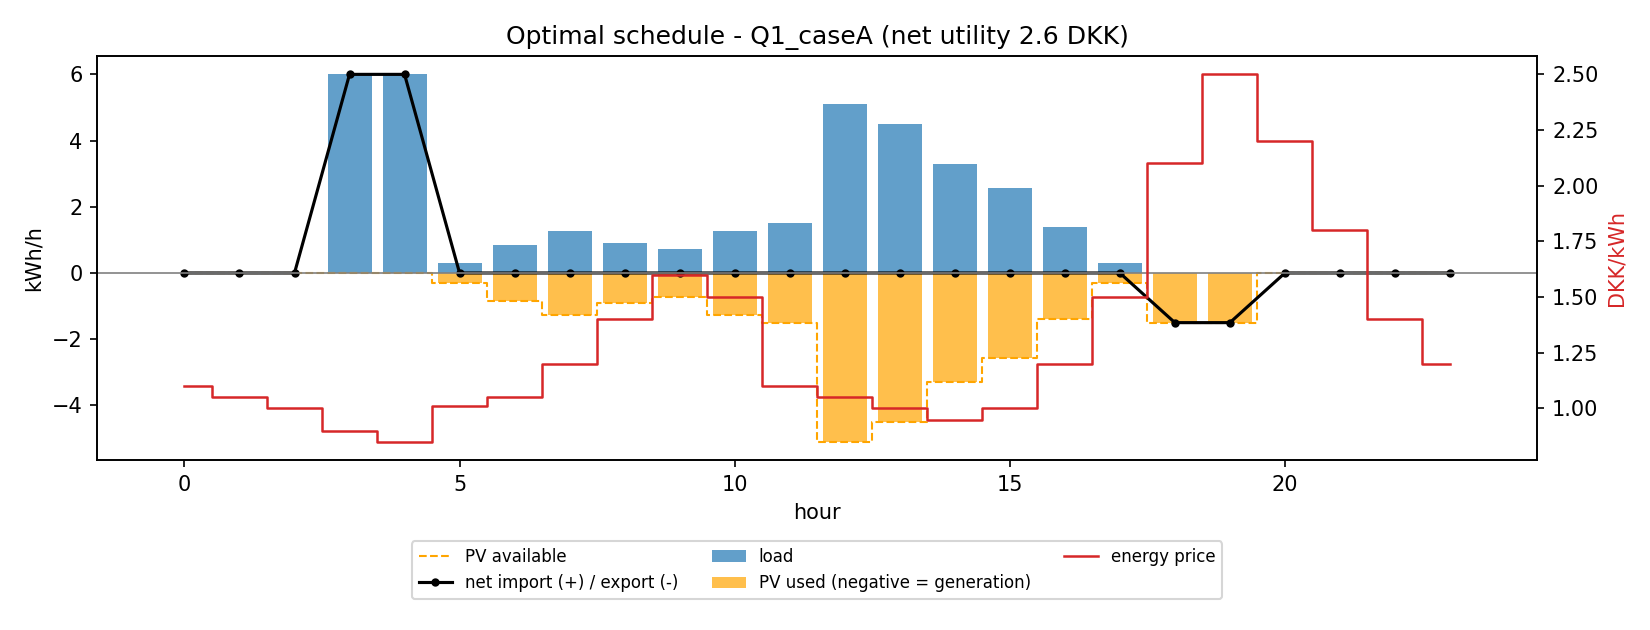
\includegraphics[width=\textwidth]{figures/Q1/schedule.png}
    \caption{Optimal schedule for case A.}
    \label{fig:q1_caseA_schedule}
\end{figure}

The case A solution gives a net utility of 2.61 DKK over the day. The consumption utility is 51.39 DKK, while the total energy cost after accounting for export revenue is 48.79 DKK.

In case A, the PV cost is $c^{PV}=1.41$ DKK/kWh, which is slightly below the consumption utility $u^L=1.43$ DKK/kWh. This makes PV worth using for own consumption in the middle of the day. In the later hours, when the export price is higher than the utility, the PV is instead sold to the grid. In total, all 26.9 kWh of available PV
is used.

The hourly behaviour in Figure~\ref{fig:q1_caseA_schedule} can be divided into four
main blocks:

\begin{itemize}
    \item \textbf{Hours 3--4 (Regime 2):} Electricity is cheap and
    $\pimp < u^L$. The load therefore reaches $L^{\max}=6$ kWh/h and
    the consumer imports.

    \item \textbf{Hours 5--17 (Regime 3):} The prices satisfy
    \[
        \pexp < u^L < \pimp.
    \]
    The consumer uses its own PV and does not trade with the grid.

    \item \textbf{Hours 18--19 (Regime 1):} Selling is more valuable than
    consuming since $\pexp > u^L$. The load is zero and all available PV
    is exported.

    \item \textbf{Hour 20 (Regime 1):} Similar as in hours 18-19, in that it is more worth to export than consuming. However in this case there is no PV, so there is nothing to export.

    \item \textbf{Hours 0--2 and 21--23 (Regime 3):} There is no PV available
    and $\pexp < u^L < \pimp$. The optimal load is therefore
    $PV_t^{\max}=0$ and there is no grid exchange.
\end{itemize}

A significant point is that no available PV is curtailed in case A. This differs from case B. If PV had been available during all hours of the day, some of it would however have been curtailed. This would happen in hours 3--4, where the PV availability is currently zero, since $c^{PV} > p_t^{imp}$. In these hours, importing electricity is cheaper than producing PV, so any available PV would be curtailed.

\paragraph{Price ladder comparison for case A}
We found that for each hour the ladder matched perfectly with the solver result for every hour in case A, meaning the predicted load and PV decisions were as expected. This can be seen in the schedule plot above and is also checked automatically in the code, which reports whether the ladder and solver results match in each hour.

\subsubsection{Case B hourly schedule}
The model was re-run for case B, now with the increased cost of PV such that it is slightly higher than the utility gain of consumption. 
\begin{figure}[H]
    \centering
    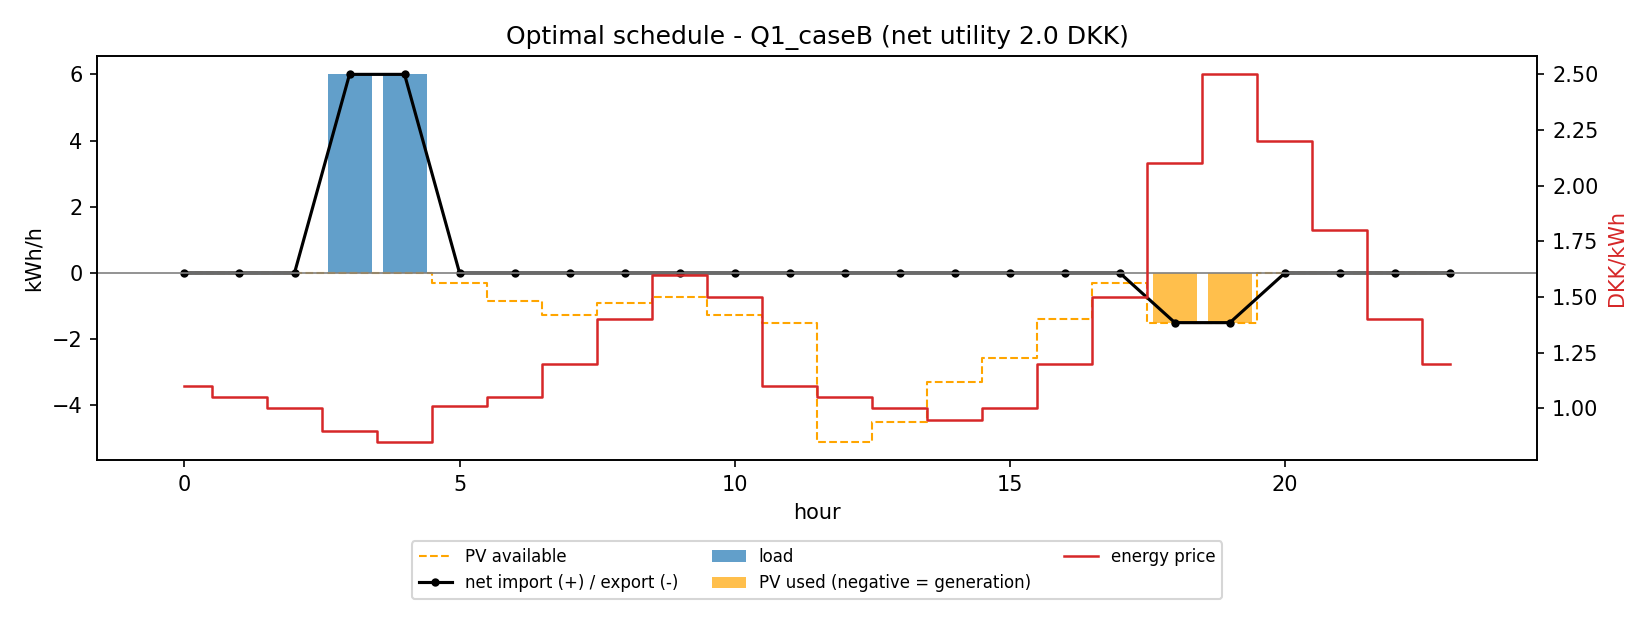
\includegraphics[width=\textwidth]{figures/Q1/scheduleB.png}
    \caption{Optimal schedule for case B.}
    \label{fig:q1_caseB_schedule}
\end{figure}
The main difference in case B compared to case A is that the PV cost has increased, such that it is now larger than the utility gain. This results in quite a significant change in behavior. The total net utility for case B is 1.95 DKK, compared to case A which had 2.61 DKK. The difference in net utility is therefore quite small, even though the PV usage changes significantly. The reason is that the gain from using PV for self-consumption in case A was only about 0.02 DKK/kWh, since $u^L-c^{PV}=1.43-1.41=0.02$. Removing this PV
consumption therefore changes the load a lot, but has only a small effect on the total net utility.

Hours 3--4 and 18--20 are unchanged from case A. The main difference appears in hours 5--17, where the most PV consumption happened in case A. Using PV for self consumption is therefore no longer worthwhile. PV is therefore only a export resource whenever that is worth it. These hours are instead idle.

Trying to fit the price ladder generated in ii-iii is less relevant here, since the regimes were generated for the case where the PV cost was below the utility gain value. This means that the price ladder is correct for regime 1 and 2, but incorrect for regime 3 where self consumption for PV is relevant. In case A, the ladder matched the solver in all 24 hours, while in case B it only matched in 11 out of 24 hours. The 13 differences occur in hours 5--17, where the ladder predicts that the load follows the available PV. In case B, these hours instead have zero load and the available PV is curtailed.

\subsubsection{Comparison of cases A and B}

Here is a quick comparison of the main numerical results for the two cases.

\begin{table}[H]
    \centering
    \begin{tabular}{lcc}
        \toprule
        & Case A & Case B \\
        \midrule
        $c^{PV}$ (DKK/kWh) & 1.41 & 1.47 \\
        Net utility (DKK) & 2.61 & 1.95 \\
        Utility / cost (DKK) & 51.39 / 48.79 & 17.16 / 15.21 \\
        Load (kWh) & 35.94 & 12.00 \\
        PV used / curtailed (kWh) & 26.94 / 0 & 3.00 / 23.94 \\
        Import / export (kWh) & 12.0 / 3.0 & 12.0 / 3.0 \\
        \bottomrule
    \end{tabular}
    \caption{Comparison of the numerical results for cases A and B.}
    \label{tab:q1_case_comparison}
\end{table}

\subsubsection{Dual variables}
The dual variables give more information about which constraints are affecting the solution in each hour, and how much they are affecting the solution. This will be looked at in detail for case A, then the main differences for case A and case B will be discussed. 

\paragraph{Case A duals}
 The below plot shows each constraint's dual value over the 24 hours for case A:

\begin{figure}[htbp]
    \centering
    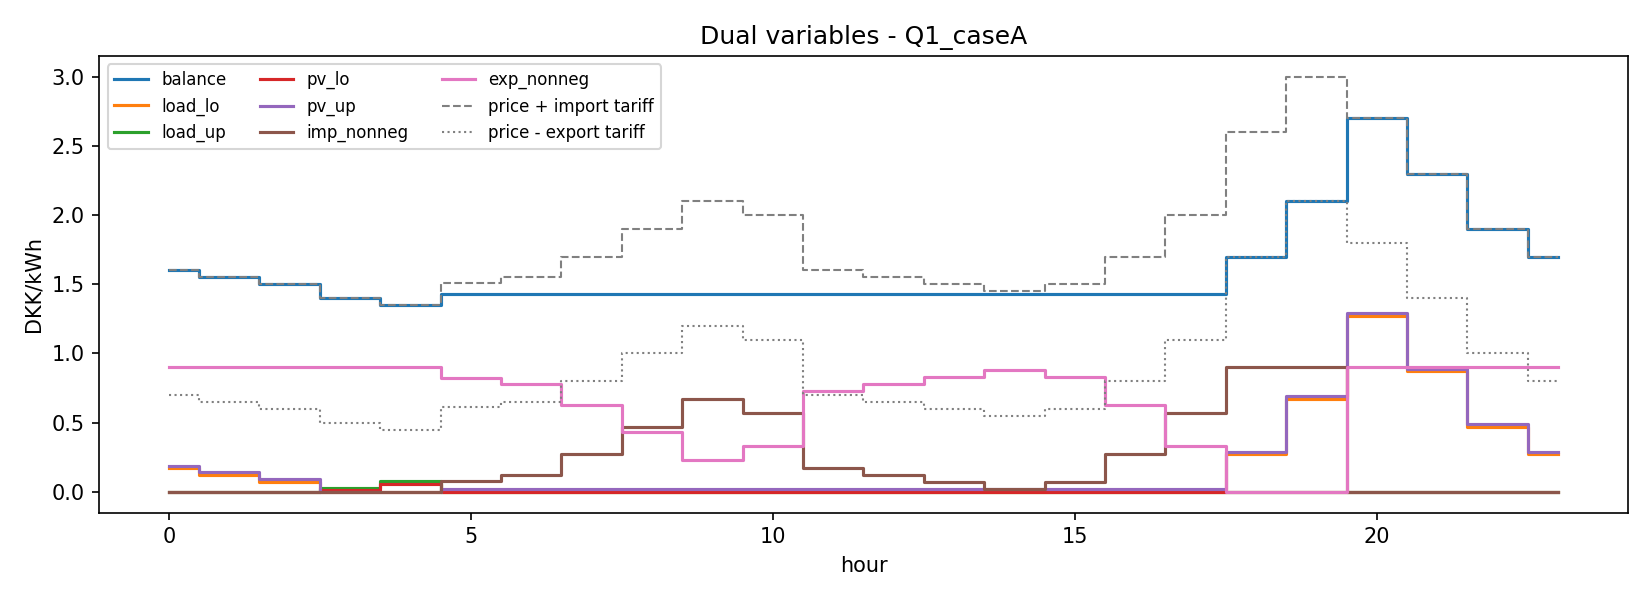
\includegraphics[width=\textwidth]{figures/Q1/duals.png}
    \caption{Duals in case A}
    \label{fig:q1_caseA_lambda_range}
\end{figure}

The table below will explain some of the trends that can be seen in the figure above: 

\small

\begin{xltabular}{\textwidth}{|p{3.2cm}|p{5cm}|X|}
\hline
\textbf{Dual (plot name)} & \textbf{Represents} & \textbf{Values in case A and what they mean} \\
\hline
\endfirsthead

\hline
\textbf{Dual (plot name)} & \textbf{Represents} & \textbf{Values in case A and what they mean} \\
\hline
\endhead

$\lambda_t$ (balance)
&
The value of one extra kWh in hour t: the consumer's internal electricity price.
&
It is set by what the consumer does with the last kWh. In hours 3-4 it buys it, so $\lambda_t$ equals the import price (1.40, 1.35). In hours 5-17 it consumes its own PV, so $\lambda_t = u^L = 1.43$. In hours 18-19 it sells it, so $\lambda_t$ equals the export price (1.70, 2.10).
\\
\hline

$\bar{\mu}^L_t$ (load\_up)
&
The gain if the consumer were allowed to consume 1 kWh more.
&
0.03 and 0.08 in hours 3-4 ($u^L - p^{imp}_t$), where import power is cheaper than the utility and the maximum load holds the consumer back. Rare situation that the import is cheaper than utility, so zero in all other hours. In the PV hours the consumer doesn't want more, since extra energy would have to be imported above 1.43.
\\
\hline

$\underline{\mu}^L_t$ (load\_lo)
&
The gain if the consumer were allowed to consume 1 kWh less.
&
0.27 and 0.67 in hours 18-19 ($p^{exp}_t - u^L$): selling a kWh pays more than consuming it, therefore the load is down to zero. So this dual is only positive when export > utility, and is the difference between the two.
\\
\hline

$\bar{\mu}^{PV}_t$ (pv\_up)
&
The value of 1 kWh more available sun.
&
0.02 in hours 5-17 ($u^L - c^{PV}$): midday sun is used for own consumption and is worth only slightly more than it costs. 0.29 and 0.69 in hours 18-19 ($p^{exp}_t - c^{PV}$). Higher values here because export prices are higher than utility usage. 
\\
\hline

$\underline{\mu}^{PV}_t$ (pv\_lo)
&
The cost of being forced to produce 1 kWh of PV.
&
The lower PV bound is zero in this model. Relaxing it further would allow negative PV production, which is not physically meaningful. It can instead be interpreted by imagining that the PV had a positive minimum production requirement. In hours 3--4, importing
electricity is cheaper than producing PV. The consumer would therefore benefit from being allowed to reduce that required PV production. The positive dual reflects the cost of being
forced to produce PV when importing would be cheaper.
\\
\hline

$\mu^{imp}_t$ (imp\_nonneg)
&
The cost of being forced to import 1 kWh.
&
It shows the cost of being forced to import when importing is not optimal. It is zero in hours 3--4, where the consumer already imports.
In hours 5--17 it is $\pimp-u^L$, and in hours 18--19 it is
$\pimp-\pexp=0.90$ DKK/kWh.
\\
\hline

$\mu^{exp}_t$ (exp\_nonneg)
&
The cost of being forced to export 1 kWh.
&
It shows the cost of being forced to export when exporting is not optimal. It is zero in hours 18--19, where the consumer already exports.
In hours 5--17 it is $u^L-\pexp$, and in hours 3--4 it is
$\pimp-\pexp=0.90$ DKK/kWh.

\\
\hline

\end{xltabular}
\paragraph{Non-unique duals}
A dual is non-unique when a small change upwards and a small change downwards give different marginal values. In that case, any value between those two can be a valid dual.

For the balance dual $\lambda_t$, this happens in the idle hours. The consumer is already at zero load then and does not trade with the grid. If a little extra energy is added through the balance, it can be consumed and is worth $u^L$ to the consumer. If energy is instead taken away, the load cannot be reduced any further. So for that reason the missing energy would have to be replaced by importing at $\pimp$. The two directions therefore have different marginal values, making $\lambda_t$ non-unique in these hours.

The same non-uniqueness also affects $\muLlo$, $\muimp$ and $\muexp$, because these duals are linked to the balance dual $\lambda_t$. For example, $\muimp=\pimp-\lambda_t$. If several values of $\lambda_t$ are valid, then several corresponding values of $\muimp$ are also valid.

The PV-bound duals $\muPVlo$ and $\muPVup$ can also be non-unique when no PV is available. The PV system has a 6 kW capacity, but the hourly upper bound is the PV that is actually available. When there is no sun the upper bound becomes zero. This forces $q_t^{PV}$ to be zero. Both PV bounds are then active at the same point. Because of this the model cannot determine one unique value for each dual.

\paragraph{Case B duals}
The dual for the constraints is plotted the same way below, but now for case B:
\begin{figure}[H]
    \centering
    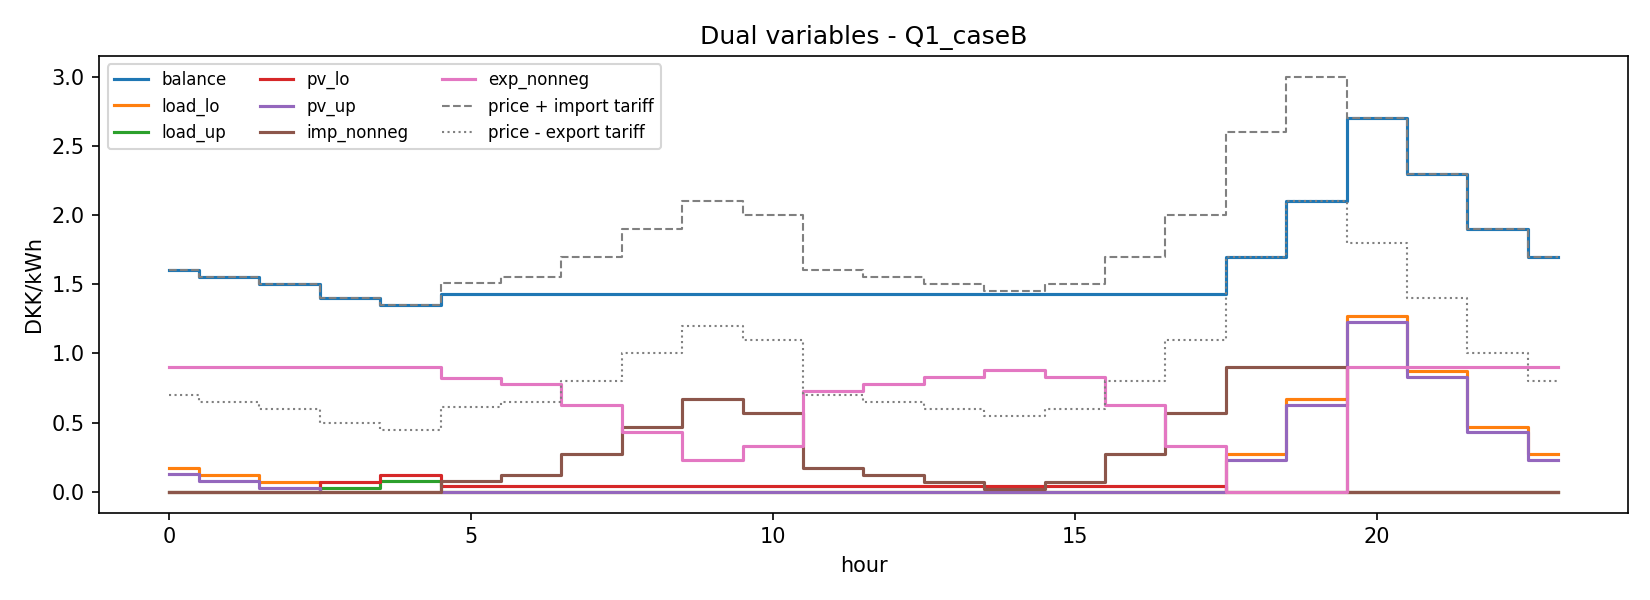
\includegraphics[width=\textwidth]{figures/Q1/dualsB.png}
    \caption{Duals for case B.}
    \label{fig:q1_caseB_lambda_range}
\end{figure}

For case B a full table like in case A would repeat a lot. Instead, just the main differences will be commented on. They all come from the higher PV cost. Most of them are in hours 5-17, where the
consumer in case B is now idle. 

\textbf{Balance ($\lambda_t$).} The value is unchanged in hours 0--4 and 18--23. In hours 5--17 Gurobi still reports 1.43 DKK/kWh, but the value is now non-unique. An extra kWh could be consumed and is therefore worth $u^L=1.43$ DKK/kWh. If energy is instead taken away, it must be replaced by PV or importing. These two directions therefore give different marginal values, showing that the dual is non-unique. 

\textbf{Load upper bound ($\muLup$).} This is unchanged compared to case A. The reason is that the PV cost does not affect the hours where the load upper bound is active.

\textbf{Load lower bound ($\muLlo$).} The only change is in hours 5--17, where the load is now at its minimum of zero. The dual depends on $\lambda_t$. Since several values of $\lambda_t$ are valid, several values of $\muLlo$ are also valid. Therefore non-unique here.

\textbf{PV upper bound ($\muPVup$).} In hours 5--17 it drops from 0.02 DKK/kWh to zero since PV is no longer worth using. In hours 18--19 it drops by 0.06 DKK/kWh. This is from the increase in PV cost.

\textbf{PV lower bound ($\muPVlo$).} In hours 5--17 it becomes positive since PV is now too expensive to use. Its value also depends on $\lambda_t$, so it is non-unique in these hours. In hours 3--4 it increases by 0.06 DKK/kWh because the PV cost has increased by the same amount.

\textbf{Import and export non-negativity ($\muimp$ and $\muexp$).} The main change is in hours 5--17. Both duals depend on $\lambda_t$, so they are also non-unique in these hours. Gurobi reports the same values as in case A because it chooses the same value $\lambda_t=1.43$ DKK/kWh.


%\todo{write for the other duals also why they are none unique.}

%load\_lo and pv\_lo follow from
%$\lambda_t$ and are not unique either. The same holds for imp\_nonneg and exp\_nonneg. For
%load\_lo and pv\_lo this has a simple meaning. Running the load on PV would lose 0.04 per kWh.
%This loss can be assigned to the load or to the PV, and Gurobi assigns it to the PV. The idle
%hours 0-2 and 20-23 are non-unique in the same way as in case A. At night the pv\_up values in
%the plot are also only Gurobi's choice. Unlike in case A, sun would not be worth using there
%except in hour 20.

%By strong duality the net utility is again the value of the binding capacities. This gives
%0.66 DKK from the load in hours 3-4 and 1.29 DKK from the evening sun. Together that is 1.95
%DKK. The sun in hours 5-17 no longer contributes, because it is no longer a binding capacity.
%As in case A, the primal solution is unique in every hour.


%Thus, a shortage is imported and a profitable surplus is exported, while an unprofitable PV surplus is curtailed.
%\todo{Summarise (ii)--(iv) as a rule: each hour the consumer compares $\uL$ and $\cpv$ with
%the two effective prices. What happens when one comparison is a tie, and what does it imply
%for the uniqueness of the primal and dual solutions? Hint: think about which multipliers or
%which primal variables can take several values when an inequality holds with equality
%(degenerate case, $\geq 0$ allowing $0$). Hint from (iii): the tie $\cpv = \pimp$ in load
%regime 2 gives partial curtailment, $0 < {\pvprod}^* < \PVmax$, and then
%${\qimp}^* = \Lmax - {\pvprod}^*$ is not unique.}

\newpage
\section{Question 2}
\subsection{(a) Generic separable disutility}

The consumer now has a preferred
consumption profile $\lref$ (kWh/h) and experiences a disutility $D_t(\load)$ (DKK) when its
load deviates from it. $D_t$ is convex, differentiable, non-negative, and equal to $0$ at
$\load = \lref$. All the other parameters, variables and constraints are those of
Question~1, and the disutility is still separable per hour.

\subsubsection{Objective function}
The term $\uL \, \load$ of \eqref{eq:daily_net_utility} is replaced by $-D_t(\load)$:
\begin{equation}
    \max_{\{\load, \qimp, \qexp, \pvprod\}_{t \in \T}} \quad
    \sum_{t \in \T} \Big( - D_t(\load) - \pimp \, \qimp + \pexp \, \qexp - \cpv \, \pvprod \Big)
    \label{eq:q2_objective}
\end{equation}
subject to the same constraints \eqref{eq:c_balance}--\eqref{eq:c_export_nonneg} as in Question~1.

\subsubsection{Properties compared with Question 1}
\begin{itemize}
    \item \textbf{Problem class and convexity:} since $D_t$ is convex, $-D_t$ is concave, so it is still a convex optimization problem, but in general no longer an LP. It
    stays an LP only if $D_t$ is piecewise linear, and becomes a QP if $D_t$ is quadratic.
    \item \textbf{Decomposability:} it still holds. $D_t$ only involves the load $\load$ of
    hour $t$, so every term of the objective and every constraint still involves a single
    hour, and the hourly decomposition argument of Question~1 applies.
    \item \textbf{Feasibility:} feasibility depends only on the constraints, not on the
    objective. Since the constraints \eqref{eq:c_balance}--\eqref{eq:c_export_nonneg} are
    exactly those of Question~1, the feasible set is unchanged, and the problem is feasible
    under the same conditions: $\Lmin \leq \Lmax$ and $\PVmax \geq 0$
    for every $t \in \T$.
\end{itemize}

\subsubsection{Question 1 as a particular case}
Choosing the constant reference $\lref = \Lmax$ and the linear disutility
\begin{equation}
    D_t(\load) = \uL \, (\Lmax - \load)
\end{equation}
gives $-D_t(\load) = \uL \, \load - \uL \, \Lmax$, that is, the objective of Question~1 up to
the constant $-24 \, \uL \, \Lmax$, which does not change the optimal solution. On the feasible
set $\load \leq \Lmax$, so $D_t \geq 0$, and $D_t = 0$ exactly at the reference. Since this expression for the disutility is linear, it means that the convex and differentiable assumptions hold, whilst it relaxes the other two.
\newline
\newline
It is non-negative only for $\load \leq \Lmax$, and becomes negative if the load exceeds the reference. It is equal to
zero at the reference, but the reference is not its minimum: $D_t$ keeps decreasing as the
load grows, and $\Lmax$ only acts as the minimum because the load bound
$\load \leq \Lmax$ stops the load there. In other words, it penalises consuming less than
the reference but would reward consuming more, instead of penalising deviations in both
directions. Both relaxed assumptions are therefore recovered only on the feasible set,
thanks to the constraint \eqref{eq:c_load_bounds}.

% ===== Question 2.(b) =====

\subsection{(b) Linear disutility}

\subsubsection{(i) Hourly disutility and LP reformulation}

The disutility is now proportional to the absolute deviation of the load from the reference,
with a coefficient $\cL > 0$ (DKK/kWh):
\begin{equation}
    D_t(\load) = \cL \, \big| \load - \lref \big|, \qquad \forall t \in \T.
    \label{eq:q2b_disutility}
\end{equation}
It is convex, non-negative and equal to zero at the reference, but at
$\load = \lref$ it is not differentiable, so the objective is no longer linear.

\paragraph{Reformulation.}
We introduce two non-negative auxiliary variables per hour: the deviation of the load above
the reference, $\dup$, and below it, $\ddn$ (both in kWh/h). They are linked to the load by
\begin{equation}
    \load - \lref = \dup - \ddn, \qquad \dup \geq 0, \quad \ddn \geq 0, \qquad \forall t \in \T,
    \label{eq:q2b_deviation}
\end{equation}
and the disutility is replaced by the linear term $\cL (\dup + \ddn)$. The hourly problem
becomes
\begin{align}
    \max_{\load,\, \qimp,\, \qexp,\, \pvprod,\, \dup,\, \ddn} \quad
    & - \cL \big( \dup + \ddn \big) - \pimp \, \qimp + \pexp \, \qexp - \cpv \, \pvprod
    \label{eq:q2b_hourly} \\
    \text{s.t.} \quad
    & \load = \pvprod + \qimp - \qexp, \nonumber \\
    & \Lmin \leq \load \leq \Lmax, \nonumber \\
    & 0 \leq \pvprod \leq \PVmax, \nonumber \\
    & \qimp \geq 0, \quad \qexp \geq 0, \nonumber \\
    & \load - \lref = \dup - \ddn, \quad \dup \geq 0, \quad \ddn \geq 0. \nonumber
\end{align}

\paragraph{Equivalence.}
For a given load, \eqref{eq:q2b_deviation} is satisfied by many pairs $(\dup, \ddn)$, and all
of them have $\dup + \ddn \geq |\load - \lref|$, with equality if and only if one of the two is
zero. An optimal solution never has both positive: if $\dup, \ddn > 0$, decreasing both by
$\varepsilon = \min(\dup, \ddn)$ keeps \eqref{eq:q2b_deviation} satisfied and increases the
objective by $2 \cL \varepsilon > 0$. Hence at the optimum $\cL(\dup + \ddn) = \cL |\load - \lref|$,
and \eqref{eq:q2b_hourly} has the same optimal load, grid exchange and objective value as the
problem with the disutility \eqref{eq:q2b_disutility}.

\paragraph{Properties.}
The objective and all the constraints are linear, so the problem is an LP, and therefore
convex. The new constraint \eqref{eq:q2b_deviation} only involves hour $t$, so the problem still
decomposes into 24 hourly problems. Each hour now has 6 variables and 10 constraints (the 7 of
Question~1, the definition of the deviation, and the non-negativity of $\dup$ and $\ddn$).

\subsubsection{(ii) Hypotheses: hourly cost-benefit argument}
In each hour, the consumer compares the cost of deviating from the reference, $\cL$ per kWh,
with what it saves on the energy it does not consume. How much it saves depends on where the
last kWh of the load comes from:
\begin{itemize}
    \item \textbf{Above the PV available} ($\load > \PVmax$), the last kWh is imported and costs
    $\pimp$.
    \item \textbf{Up to the PV available} ($\load \leq \PVmax$), it comes from the consumer's own
    PV. A kWh of PV that is not consumed is either exported, earning $\pexp$, or curtailed,
    saving $\cpv$, whichever is better. Consuming it therefore costs
    \begin{equation}
        \mPV = \max\big(\cpv, \pexp\big),
        \label{eq:q2b_mpv}
    \end{equation}
    assuming $\cpv < \pimp$ (otherwise the PV is never used, and every kWh costs $\pimp$). Since
    $\pexp < \pimp$, we have $\mPV \leq \pimp$.
\end{itemize}
The marginal cost of supplying the load is thus a step function of the load: $\mPV$ up to
$\PVmax$, then $\pimp$.

\paragraph{Consumption above the reference.}
We expect the load never to exceed its reference. Consuming one kWh above $\lref$ costs energy
($\cpv$, $\pexp$ and $\pimp$ are all positive, the last two because $p_t > \tauexp$) and adds a
disutility $\cL > 0$, with no benefit in return. Unlike Question~1, a kWh consumed has no value
in itself; it only has value as a way of reducing the deviation from the reference.

\paragraph{Gradual response or jumps.}
Both the marginal cost of deviating ($\cL$) and the marginal saving ($\mPV$ or $\pimp$) are
constant within each segment of the load. Within a segment, the consumer therefore either
deviates as much as possible or not at all. We expect the load to jump between at most three
candidate values, with thresholds on $\cL$:
\begin{center}
\small
\begin{tabularx}{\textwidth}{llX}
    \toprule
    Condition & Optimal load ${\load}^*$ & Interpretation \\
    \midrule
    $\cL > \pimp$ & $\lref$ & following the reference is worth even importing \\
    $\mPV < \cL < \pimp$ & $\max\big(\Lmin, \min(\PVmax, \lref)\big)$ & consume only what the own PV covers \\
    $\cL < \mPV$ & $\Lmin$ & not even the own PV is worth consuming \\
    \bottomrule
\end{tabularx}
\end{center}
If $\lref \leq \PVmax$, the first two rows coincide and there are only two candidate values,
separated by $\mPV$. When $\cL$ is exactly equal to a threshold, the consumer is indifferent, and
any load between the two neighbouring candidate values is optimal. The load is then not
unique. The deviation is limited by the load bound only in the last row (${\load}^* = \Lmin$).

For the day as a whole, $\cL$ is the same in every hour, but the thresholds are not, since the
prices change from hour to hour. The daily consumption should therefore increase with $\cL$ in
steps, one each time $\cL$ crosses the threshold of some hour. In the base case,
$\pexp < \cpv$ in almost every hour, so $\mPV = \cpv$ in most hours, and we expect one large jump
at $\cL = \cpv$.

\subsubsection{(iii) Implementation}
The model is the class \texttt{LinearDisutilityModel} in \texttt{src/model.py}. It extends \texttt{DisutilityModel}, a subclass of the Question~1 model (\texttt{FlexibleConsumerModel}) that builds all its variables and constraints with a zero utility and replaces the objective by the
disutility and the procurement cost. \texttt{LinearDisutilityModel} only adds the deviation variables and the constraint \eqref{eq:q2b_deviation}, so the objective is \eqref{eq:q2b_hourly} summed over the 24 hours. The function \texttt{run\_q2\_sweep} in \texttt{main.py} runs the base case
and the sweep of (iv), writes the results to \texttt{results/Q2\_linear/} and the figures to \texttt{report/figures/}, and checks the hypotheses of (ii) on every run (\texttt{python main.py --question Q2\_linear --sweep}).

\subsubsection{(iv) Numerical results}

\paragraph{Base case.}
In the base case, $\cL = 1.43$~DKK/kWh, just above $\cpv = 1.41$~DKK/kWh and below the import
price of every hour ($\pimp \geq 1.45$~DKK/kWh in the hours with a positive reference). According
to (ii), the load should cover the reference with the own PV only, and never import.
Figure~\ref{fig:q2b_schedule} shows the result:

\begin{figure}[H]
    \centering
    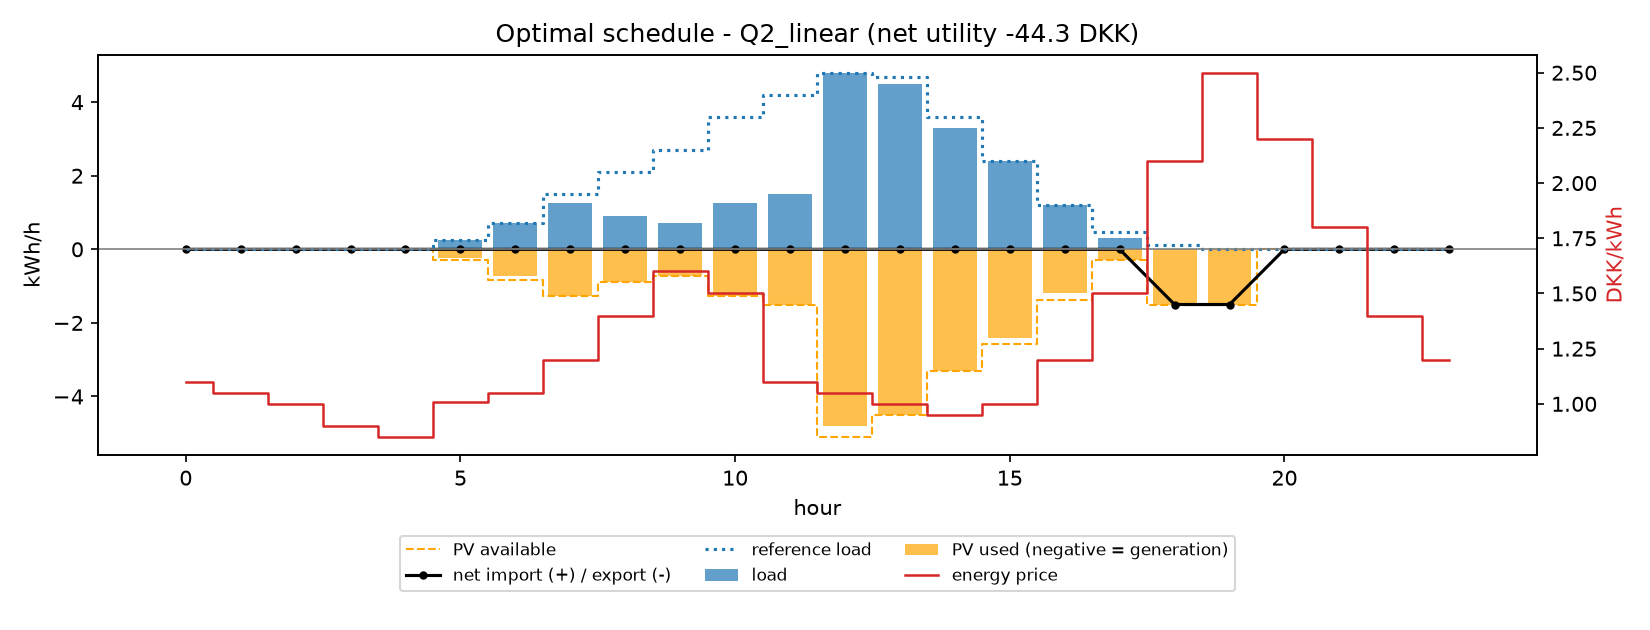
\includegraphics[width=\textwidth]{figures/Q2/q2b_schedule.png}
    \caption{Base case of the linear disutility model ($\cL = 1.43$~DKK/kWh). Blue bars: optimal load; dotted line: reference load. Orange bars (negative): PV used; dashed orange line: PV available. Black line: net import ($+$) or export ($-$). Red line: energy price (right axis).}
    \label{fig:q2b_schedule}
\end{figure}

\begin{itemize}
    \item In the hours where the PV covers the reference (hours 5, 6, 12, 15 and 16), the load
    follows it exactly. The PV left over is curtailed (0.84~kWh in total), since exporting it
    pays less than it costs to produce ($\pexp < \cpv$).
    \item In the hours where the reference exceeds the PV (hours 7--11, 13, 14 and 17), the load
    is cut down to the PV available. Importing the rest would cost $\pimp > \cL$.
    \item In hour 18, the load drops to zero, although the PV would cover the reference: here
    $\pexp = 1.70 > \cL$, so exporting the PV is worth more than consuming it. This is the only
    hour where the deviation is limited by the load bound.
\end{itemize}
Over the day, the consumer consumes 23.1~kWh instead of 32.3~kWh (total absolute deviation
9.24~kWh), does not import at all, and exports 3.0~kWh in hours 18 and 19. The procurement cost is
31.10~DKK and the disutility 13.21~DKK.

\paragraph{Sweep over $\cL$.}
The model is solved for $\cL$ from 0.005 to 3.195~DKK/kWh in steps of 0.01~DKK/kWh. The grid is
offset by 0.005 so that no run falls exactly on a price threshold, where the solution would not
be unique. The load changes only at a few values of $\cL$ (Figure~\ref{fig:q2b_sweep}), and
Table~\ref{tab:q2b_sweep} reports one run in each of the resulting intervals.

\begin{table}[H]
    \centering
    \small
    \begin{tabular}{lcrrrrr}
        \toprule
        Interval of $\cL$ & $\cL$ & Cost & Disutility & Energy & $\sum_t |\load - \lref|$ & Hours at \\
        (DKK/kWh) & (DKK/kWh) & (DKK) & (DKK) & (kWh) & (kWh) & bound \\
        \midrule
        $< 1.41$      & 1.000 & $-1.47$ & 32.34 & 0.00  & 32.34 & 14 \\
        $1.41$--$1.45$ & 1.430 & 31.10 & 13.21 & 23.10 & 9.24  & 1 \\
        $1.45$--$1.50$ & 1.475 & 31.54 & 13.19 & 23.40 & 8.94  & 1 \\
        $1.50$--$1.60$ & 1.550 & 31.81 & 13.58 & 23.58 & 8.76  & 1 \\
        $1.60$--$1.70$ & 1.650 & 36.13 & 10.00 & 26.28 & 6.06  & 1 \\
        $1.70$--$1.90$ & 1.800 & 36.74 & 10.26 & 26.64 & 5.70  & 0 \\
        $1.90$--$2.00$ & 1.950 & 39.02 & 8.78  & 27.84 & 4.50  & 0 \\
        $2.00$--$2.10$ & 2.050 & 44.06 & 4.06  & 30.36 & 1.98  & 0 \\
        $> 2.10$      & 2.500 & 48.22 & 0.00  & 32.34 & 0.00  & 0 \\
        \bottomrule
    \end{tabular}
    \caption{Sweep over $\cL$: one run in each interval between two consecutive change points.
    Cost: daily procurement cost; energy: daily energy consumed; hours at bound: hours in which
    the deviation is limited by the load bound ($\load = \Lmin$ while $\lref > \Lmin$).}
    \label{tab:q2b_sweep}
\end{table}

\begin{figure}[H]
    \centering
    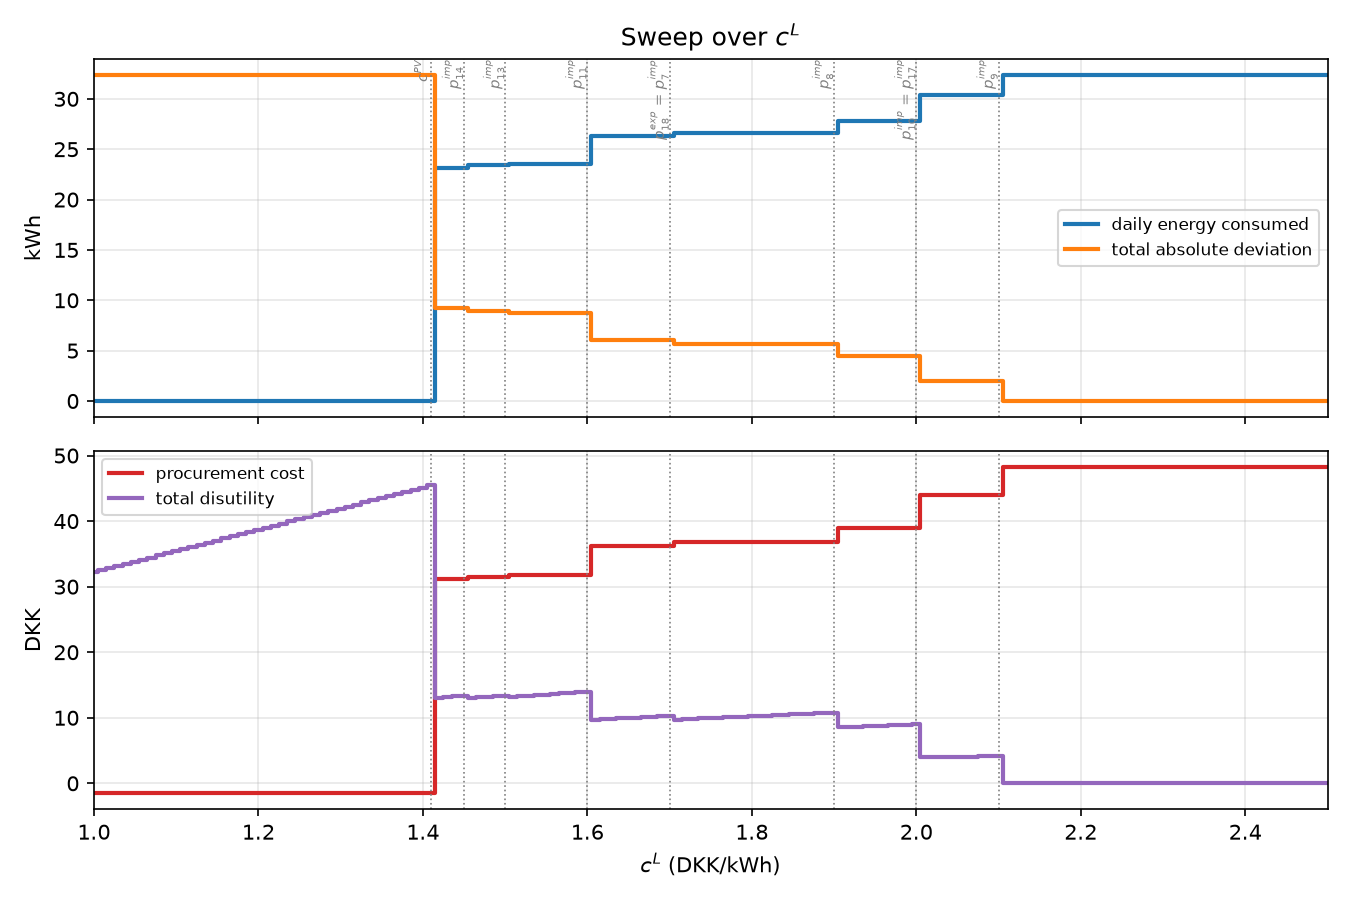
\includegraphics[width=0.9\textwidth]{figures/Q2/q2b_sweep.png}
    \caption{Sweep over $\cL$. Top: daily energy consumed and total absolute deviation. Bottom:
    procurement cost and total disutility. The dotted lines mark the thresholds predicted in
    (ii). The plot is restricted to $1 \leq \cL \leq 2.5$~DKK/kWh; nothing changes outside it.}
    \label{fig:q2b_sweep}
\end{figure}

\paragraph{Change points.}
The behaviour changes at exactly the thresholds predicted in (ii):
\begin{itemize}
    \item \textbf{$\cL < \cpv = 1.41$:} the consumer consumes nothing, in all 14 hours with a
    positive reference, and the deviation is limited by the load bound in all of them. The PV is
    used only in hours 18 and 19, where exporting it pays more than it costs
    ($\pexp > \cpv$), which gives a negative procurement cost (a net revenue of 1.47~DKK).
    \item \textbf{$\cL = \cpv$:} the large jump. In hours 5--17, $\mPV = \cpv$, and the load jumps
    from zero to the PV available or to the reference, whichever is smaller (from 0 to
    23.1~kWh per day).
    \item \textbf{$\cpv < \cL < 2.10$:} each further step happens when $\cL$ crosses the import
    price of an hour whose reference exceeds the PV: $\pimp$ of hours 14 (1.45), 13 (1.50),
    11 (1.60), 7 (1.70), 8 (1.90), 10 and 17 (2.00) and 9 (2.10). At that point the load of that
    hour jumps to its reference and the difference is imported. At $\cL = 1.70$, hour 18 also
    switches, since $\mPV = \pexp = 1.70$ there: its reference is now consumed from the PV instead
    of exporting it.
    \item \textbf{$\cL > 2.10$:} the load follows the reference exactly in every hour, and
    9.12~kWh are imported.
\end{itemize}
The procurement cost increases with $\cL$, in steps. The disutility does not: within an
interval the deviation is fixed and the disutility grows linearly with $\cL$, and at each change
point the deviation drops and the disutility falls. This gives the saw-tooth shape of
Figure~\ref{fig:q2b_sweep}.

\paragraph{Hypotheses of (ii).}
The results confirm them:
\begin{itemize}
    \item The load is never above the reference, in any hour of any run.
    \item The load does not vary gradually with $\cL$. It is piecewise constant, and in every hour
    it takes one of the three candidate values $\lref$, $\min(\PVmax, \lref)$ or $\Lmin$. The
    hourly loads of all runs match the rule of the table in (ii) exactly.
    \item The daily consumption increases in steps, with the largest step at $\cL = \cpv$.
\end{itemize}

% ===== Question 2.(c) =====

\subsection{(c) Quadratic disutility}

\subsubsection{(i) Hourly problem and its class}

The disutility is now quadratic in the deviation from the reference, with a coefficient
$\cQ > 0$ (DKK/kWh$^2$):
\begin{equation}
    D_t(\load) = \cQ \, \big( \load - \lref \big)^2, \qquad \forall t \in \T.
    \label{eq:q2c_disutility}
\end{equation}
Unlike \eqref{eq:q2b_disutility}, $D_t$ is differentiable everywhere, including at the
reference, so no reformulation is needed: the hourly problem is directly
\begin{align}
    \max_{\load,\, \qimp,\, \qexp,\, \pvprod} \quad
    & - \cQ \big( \load - \lref \big)^2 - \pimp \, \qimp + \pexp \, \qexp - \cpv \, \pvprod
    \label{eq:q2c_hourly} \\
    \text{s.t.} \quad
    & \load = \pvprod + \qimp - \qexp, \nonumber \\
    & \Lmin \leq \load \leq \Lmax, \nonumber \\
    & 0 \leq \pvprod \leq \PVmax, \nonumber \\
    & \qimp \geq 0, \quad \qexp \geq 0. \nonumber
\end{align}

\paragraph{Properties.}
\begin{itemize}
    \item \textbf{Problem class and convexity:} $D_t$ is a quadratic function of $\load$ with
    coefficient $\cQ > 0$, so $-D_t$ is strictly concave, and \eqref{eq:q2c_hourly} maximizes a
    strictly concave function over the same polyhedron as in Question~2.(a): a strictly convex
    Quadratic Program (QP).
    \item \textbf{Decomposability:} it still holds, for the same reason as 2.(a) and 2.(b):
    $D_t$ only involves the load of hour $t$, so the problem decomposes into 24 hourly QPs.
    \item \textbf{Uniqueness:} because $D_t$ is strictly convex, each hour's optimal load is the unique optmial value that can be obtained. In the linear disutility case, a price landing exactly on the threshold $\cL$ made every load on the flat part of $D_t$'s slope equally optimal.
\end{itemize}

\subsubsection{(ii) Hypotheses: first-order condition}

Writing the stationarity condition of \eqref{eq:q2c_hourly} with respect to $\load$, with $\lbal$ the multiplier of the balance constraint \eqref{eq:c_balance}:
\begin{equation}
    \frac{\partial}{\partial \load} \Big[ -\cQ (\load - \lref)^2 \Big] = \lbal 
    \quad\Longrightarrow\quad
    \load^\star = \lref - \frac{\lbal}{2 \cQ},
    \label{eq:q2c_foc}
\end{equation}

with the $\load^\star$ symbol meaning it is the optimal load. As in 2.(b), $\lbal$ equals $\pimp$ if the load is above the PV available, and equals $\mPV = \max(\cpv, \pexp)$ if the load is at or below the PV available.

\paragraph{Consumption above the reference.}
The consumer never uses more than its reference in any hour. Consuming more than the reference would make no sense for two reasons: it costs money, and it brings no benefit either, because in this model any deviation from the reference, upwards or downwards, only adds disutility. So going above the reference means paying more and also being less comfortable.

In mathematical terms; \eqref{eq:q2c_foc} gives $\load^\star = \lref - \lbal/(2\cQ)$, where $\lbal$ is the marginal cost of one more kWh in that hour. Going above the reference ($\load^\star > \lref$) would need $\lbal < 0$, i.e.\ a negative cost of energy, so that the consumer is paid to consume. But $\lbal$ is either $\pimp$ or $\mPV$, and both are strictly positive. Hence $\load^\star \leq \lref$ in every hour, for any $\cQ > 0$. This is the same conclusion as in 2.(b).ii, now obtained directly from \eqref{eq:q2c_foc}.

\paragraph{Gradual response, not jumps.}
Unlike 2.(b), where the load jumped between at most three fixed values as $\cL$ crossed a threshold, \eqref{eq:q2c_foc} is continuous and strictly monotonic in both $\lbal$ and $\cQ$: there is no finite jump in $\load^\star$ for any finite change in the price or in $\cQ$. 

\paragraph{Closed form, combining both.} Writing out the two regimes of $\lbal$ explicitly:
\begin{equation}
    \load^\star = \mathrm{clip}\!\left(
    \begin{cases}
        \lref - \dfrac{\pimp}{2\cQ} & \text{if this exceeds } \PVmax \quad (\text{importing}) \\[6pt]
        \lref - \dfrac{\mPV}{2\cQ} & \text{if this is below } \PVmax \quad (\text{own PV only}) \\[6pt]
        \PVmax & \text{otherwise (neither rule is self-consistent)}
    \end{cases}, \;\; \Lmin, \;\; \Lmax \right)
    \label{eq:q2c_closed_form}
\end{equation}
Same two marginal-cost regimes as the threshold rule of 2.(b), but with a continuous interior solution within each regime instead of a single flat value.

\subsubsection{(iii) Implementation}
The model is the class \texttt{QuadraticDisutilityModel} in \texttt{src/model.py}. Like \texttt{LinearDisutilityModel}, it extends \texttt{DisutilityModel} and only defines the disutility, so the objective is \eqref{eq:q2c_hourly} summed over the 24 hours. No auxiliary variables are needed, since the square in \eqref{eq:q2c_disutility} is passed to Gurobi directly as a quadratic objective. The base case, the sweep and the checks of (iv) are run by \texttt{run\_q2\_sweep} (\texttt{python main.py --question Q2\_quadratic --sweep}).

\subsubsection{(iv) Numerical results}

\paragraph{Base case.} With $\cQ = 1.00$~DKK/kWh$^2$ (Figure~\ref{fig:q2c_schedule}):
\begin{itemize}
    \item The load never exceeds the reference (hypothesis of (ii)).
    \item Hours 5, 17 and 18 sit at $\Lmin = 0$; in every other hour with a positive reference the
    load is an interior solution of \eqref{eq:q2c_foc}.
    \item In hours 8--11 the model imports part of the shortfall (4.42~kWh in total) instead of
    cutting the load down to the PV available.
\end{itemize}
Over the day the consumer uses 22.8~kWh (reference: 32.3~kWh), with $\sum_t|\load-\lref| =
9.57$~kWh, 4.42~kWh imported and 3.00~kWh exported. The procurement cost is 32.54~DKK and the
disutility 7.43~DKK.

\begin{figure}[H]
    \centering
    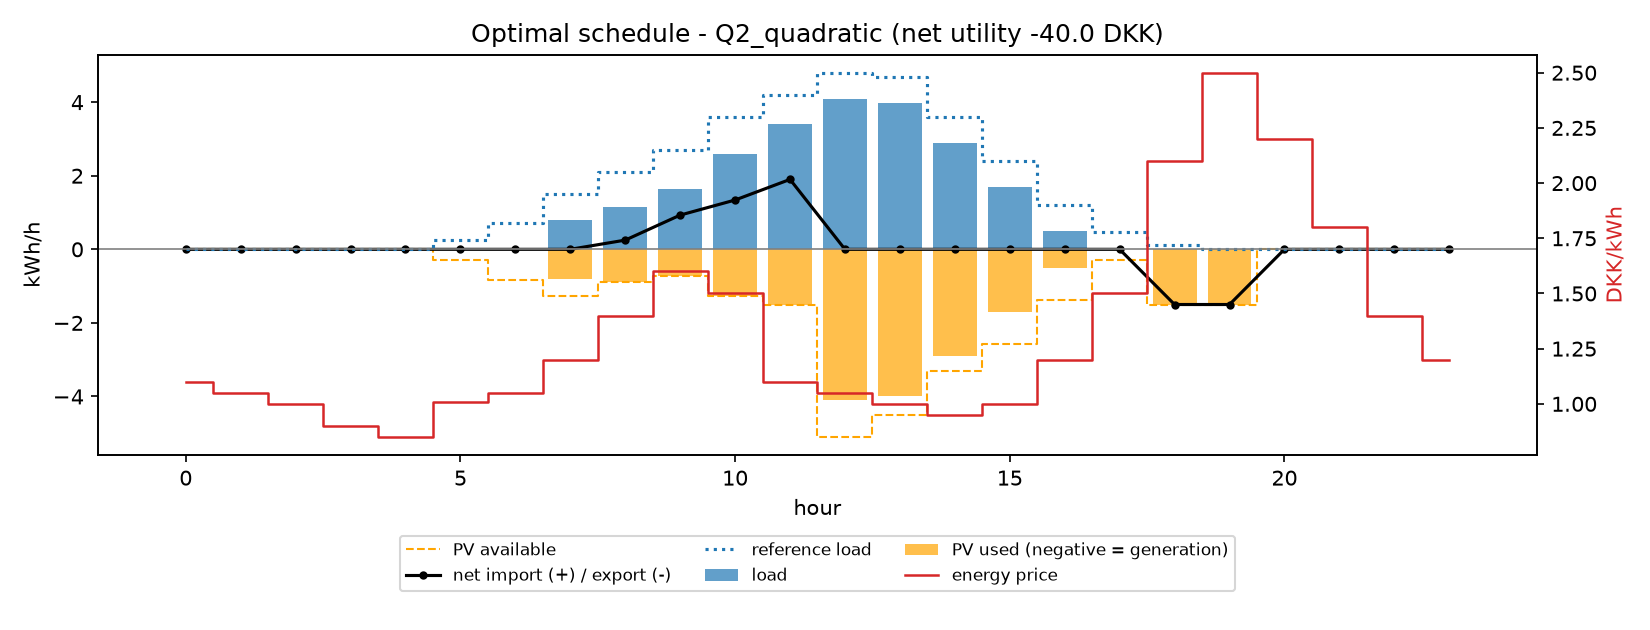
\includegraphics[width=\textwidth]{figures/Q2/q2c_schedule.png}
    \caption{Base case of the quadratic model ($\cQ = 1.00$~DKK/kWh$^2$). Same legend as Figure~\ref{fig:q2b_schedule}.}
    \label{fig:q2c_schedule}
\end{figure}

\paragraph{Sweep over $\cQ$.} The model is solved for $\cQ$ from 0.01 to 3.20 in steps of 0.01.
Table~\ref{tab:q2c_sweep} shows a selection and Figure~\ref{fig:q2c_sweep} the full sweep. Unlike
2.(b), every value of $\cQ$ gives a different load profile and all curves are smooth.

\begin{table}[H]
    \centering
    \small
    \begin{tabular}{crrrrrr}
        \toprule
        $\cQ$ & Cost & Disutility & Energy & $\sum_t |\load - \lref|$ & Import & Hours at \\
        (DKK/kWh$^2$) & (DKK) & (DKK) & (kWh) & (kWh) & (kWh) & bound \\
        \midrule
        0.20 &  3.12 & 16.82 &  3.26 & 29.08 & 0.00 & 9 \\
        0.50 & 20.85 & 12.33 & 15.54 & 16.80 & 1.44 & 5 \\
        1.00 & 32.54 &  7.43 & 22.77 &  9.57 & 4.42 & 3 \\
        1.43 & 36.83 &  5.41 & 25.39 &  6.95 & 5.56 & 3 \\
        2.00 & 39.85 &  3.95 & 27.26 &  5.08 & 6.32 & 2 \\
        3.00 & 42.38 &  2.77 & 28.83 &  3.51 & 7.01 & 1 \\
        \bottomrule
    \end{tabular}
    \caption{Sweep over $\cQ$ (selected runs). "Hours at bound" counts the hours where the load
    sits at $\Lmin$ while deviating from the reference.}
    \label{tab:q2c_sweep}
\end{table}

\begin{figure}[H]
    \centering
    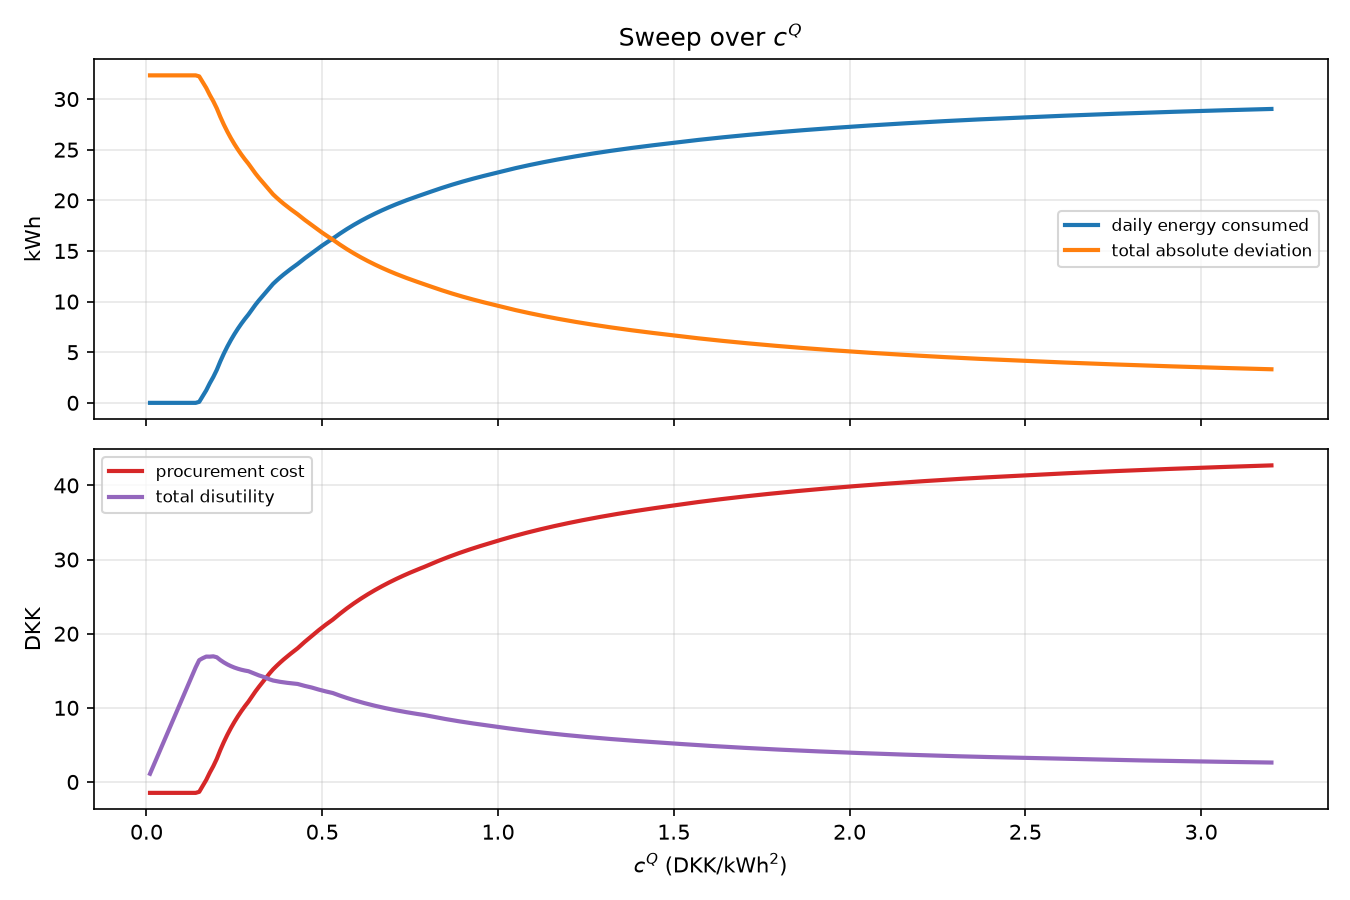
\includegraphics[width=0.9\textwidth]{figures/Q2/q2c_sweep.png}
    \caption{Sweep over $\cQ$. Top: daily energy and total absolute deviation. Bottom:
    procurement cost and total disutility. Compare with Figure~\ref{fig:q2b_sweep}: no flat
    segments or jumps.}
    \label{fig:q2c_sweep}
\end{figure}

\paragraph{Comparison with 2.(b).} At $\cL = \cQ = 1.43$:
\begin{center}
\small
\begin{tabular}{lrrrr}
    \toprule
    Model & Energy (kWh) & $\sum_t |\load - \lref|$ (kWh) & Disutility (DKK) & Cost (DKK) \\
    \midrule
    Linear    & 23.10 & 9.24 & 13.21 & 31.10 \\
    Quadratic & 25.39 & 6.95 &  5.41 & 36.83 \\
    \bottomrule
\end{tabular}
\end{center}
The quadratic consumer deviates less and imports more: instead of cutting down to the PV
available (corner solution of the linear model), it imports a little in each PV-constrained hour
and balances the marginal disutility against the price.

\paragraph{Checks.}
\begin{itemize}
    \item The load never exceeds the reference in any run of the sweep.
    \item The load matches \eqref{eq:q2c_closed_form} in every hour and run to within
    $5\times10^{-4}$~kWh.
    \item The response is smooth: the largest change in one hour for a $\cQ$ step of 0.01 is
    0.29~kWh, against the 2--5~kWh jumps of Table~\ref{tab:q2b_sweep}.
    \item Re-solving the base case with a different Gurobi seed gives the same load profile,
    consistent with the uniqueness argued in (i).
\end{itemize}

% ===== Question 2.(d) =====

\subsection{(d) Multi-model comparison}

\paragraph{Scenarios.} We compare the base case and two scenarios, solved with both models at the same coefficient value: a low value ($\cL = \cQ = 0.50$) and a high value
($\cL = \cQ = 3.20$), both taken from the sweeps of (b).iv and (c).iv. The base case uses $\cL = 1.43$~DKK/kWh and $\cQ = 1.00$~DKK/kWh$^2$. The two coefficients have different units,
so equal values are not equal discomfort; they only give two comparable points on each sweep. As a reference we also solve the Question 1 model (linear utility $u^L = \cL$, no reference
profile) on the same prices and PV. Results are in Table~\ref{tab:q2d_comparison} and Figure~\ref{fig:q2d_profiles}.

\begin{table}[H]
    \centering
    \small
    \begin{tabular}{llrrrrrr}
        \toprule
        Scenario & Model & Cost & Energy & $\sum_t |\load - \lref|$ & Import & Hours & Hours \\
                 &       & (DKK) & (kWh) & (kWh) & (kWh) & at ref. & at 0 \\
        \midrule
        Base & Q1 utility & 48.79 & 35.94 & 22.08 & 12.00 & 0 & 1 \\
             & Linear     & 31.10 & 23.10 &  9.24 &  0.00 & 5 & 1 \\
             & Quadratic  & 32.54 & 22.77 &  9.57 &  4.42 & 0 & 3 \\
        \midrule
        Low ($c = 0.50$)  & Q1 utility &  -1.47 &   0.00 &  32.34 &   0.00 & 0 & 14 \\
                          & Linear     &  -1.47 &   0.00 &  32.34 &   0.00 & 0 & 14 \\
                          & Quadratic  &  20.85 &  15.54 &  16.80 &   1.44 & 0 &  5 \\
        \midrule
        High ($c = 3.20$) & Q1 utility & 253.25 & 144.00 & 111.66 & 117.06 & 0 &  0 \\
                          & Linear     &  48.22 &  32.34 &   0.00 &   9.12 & 14 & 0 \\
                          & Quadratic  &  42.70 &  29.02 &   3.32 &   7.11 & 0 &  1 \\
        \bottomrule
    \end{tabular}
    \caption{Comparison of the three models for eahc scenario "Hours at ref." counts the hours with a positive reference where the load equals the reference; "Hours at 0" those where it is zero despite a positive reference. The Q1 model has no reference, so its deviation is only a reference
    point.}
    \label{tab:q2d_comparison}
\end{table}

\begin{figure}[H]
    \centering
    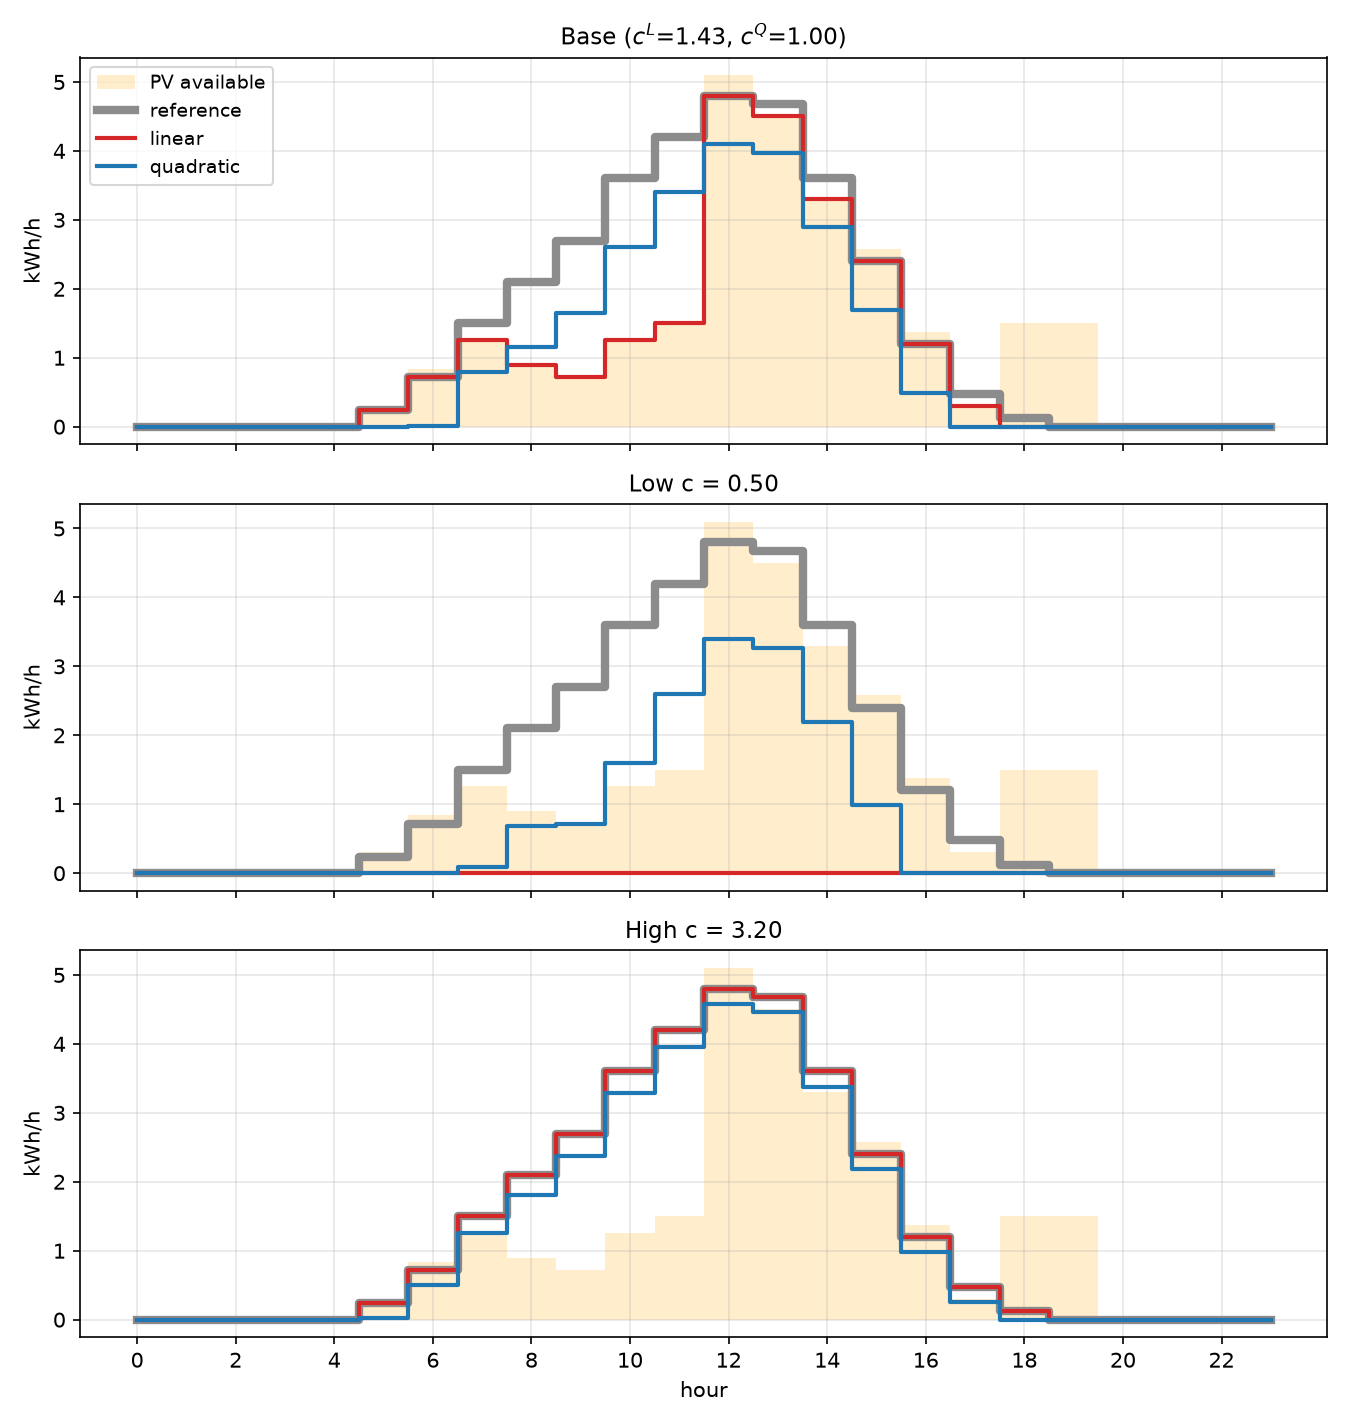
\includegraphics[width=0.85\textwidth]{figures/Q2/q2d_profiles.png}
    \caption{Load profiles of the linear and quadratic models against the reference and the PV available, for the base case and the two scenarios.}
    \label{fig:q2d_profiles}
\end{figure}

\paragraph{Analysis.}
\begin{itemize}
    \item \textbf{Linear: three regimes.} Depending on $\cL$, the load is zero (low), equal to the PV available (middle) or equal to the reference (high). At $\cL = 0.50$ it consumes nothing, at 1.43 it cuts the load down to the PV available (no import, 5 hours exactly at the reference), and at 3.20 it follows the reference in all 14 active hours (Table~\ref{tab:q2d_comparison}).
    \item \textbf{Quadratic: gradual.} The same change in $\cQ$ moves the load a little in every hour: 15.5~kWh at 0.50, 22.8~kWh at 1.00 and 29.0~kWh at 3.20, and the load is never exactly at the reference. It always imports a bit (1.4 to 7.1~kWh) instead of choosing between ``PV only'' and ``everything''.
    \item \textbf{Q1 model.} At low $c$ it coincides with the linear model (nothing is worth consuming). With no reference, at higher $c$ it consumes the maximum in every hour (144~kWh at 3.20), which is why the reference-based models are needed for a realistic profile.
    \item \textbf{Cost vs deviation.} In the base case the two models cost about the same (31.10 vs 32.54~DKK) and deviate by about the same (9.24 vs 9.57~kWh), but in different hours and in a different way: the linear one deviates a lot in few hours, the quadratic one a little in many hours.
\end{itemize}

\paragraph{Why corner solutions vs a gradual response.} In each hour the consumer compares the marginal disutility of deviating with the marginal cost of energy. For the linear model the marginal disutility is the constant $\cL$ at every deviation, so the comparison with the price has the same answer for every kWh: either all of it is worth consuming or none of it, and the
load jumps to a corner whenever $\cL$ crosses a price. For the quadratic model the marginal disutility $2\cQ|\load - \lref|$ grows with the deviation, so the first kWh of deviation is
nearly free and the last is very costly; the optimum is where it equals the price \eqref{eq:q2c_foc}, which moves continuously with $\cQ$ and the prices.

\paragraph{Recommendation.} The linear disutility fits loads that are either worth using or not at a given price (a deferrable process, charging that can be shifted or skipped): the consumer only has to state one number, a price threshold, and gets an on/off response, which is easy to predict but abrupt and sensitive to price changes at the thresholds. The quadratic disutility fits comfort-driven loads (heating, lighting) where small deviations are tolerated and large ones are increasingly unpleasant: it gives a smooth, stable response, but the consumer has to express how bad a deviation of each size is (a curvature, in DKK/kWh$^2$), which is harder to state in practice.

% ===== Question 2.(e) (bonus) =====

\subsection{(e) Non-separable disutility}

\subsubsection{(i) Formulation and properties}

In real life it is the case that we do not consider each hour on its own, rather we feel the discomfort as consumers when we are off the reference load for multiple consecutive hours. A way to model this is with an accumulated deviation that fades over time; let $\Delta_t = \load - \lref$ be the deviation of hour $t$, and $e_t$ the accumulated deviation (kWh), with a memory factor $\rho \in [0,1]$:
\begin{equation}
    e_t = \rho \, e_{t-1} + \Delta_t, \qquad \forall t \in \T, \qquad e_{-1} = 0.
    \label{eq:q2e_state}
\end{equation}
A deviation in one hour fades by a factor $\rho$ every hour, while deviations in consecutive hours add up. The disutility of the whole day is
\begin{equation}
    D(\boldsymbol{\ell}) = \sum_{t \in \T} \Big( \cQ \, \Delta_t^2 + \cS \, e_t^2 \Big),
    \qquad \cQ \geq 0, \;\; \cS > 0.
    \label{eq:q2e_disutility}
\end{equation}
The first term is the hourly discomfort of 2.(c); the second penalizes accumulated deviations. For example, with $\rho = 0.5$ a deviation of 1~kWh in three consecutive hours gives $7.33$, while three isolated deviations of 1~kWh give $3 \times 1.33 = 4.00$: the same total deviation is penalized more when it is sustained. The problem is
\begin{align}
    \max_{\load,\, \qimp,\, \qexp,\, \pvprod,\, e_t} \quad
    & - D(\boldsymbol{\ell}) - \sum_{t \in \T} \Big( \pimp \, \qimp - \pexp \, \qexp + \cpv \, \pvprod \Big)
    \label{eq:q2e_problem} \\
    \text{s.t.} \quad
    & \text{the constraints of Question~1 for every } t \in \T, \nonumber \\
    & e_t = \rho \, e_{t-1} + \load - \lref, \quad \forall t \in \T. \nonumber
\end{align}

\paragraph{Properties.}
\begin{itemize}
    \item \textbf{Convexity and class:} $D$ is a sum of squares of linear functions of the loads, so it is convex, and \eqref{eq:q2e_problem} maximizes a concave function over a polyhedron: a Quadratic Program (QP). With $\cQ > 0$ it is strictly concave in the loads.
    \item \textbf{Decomposability:} it is lost. $\load$ appears in $e_t, e_{t+1}, \dots$ through \eqref{eq:q2e_state}, so the disutility couples the hours and the problem is a single
    24-hour QP, with 24 additional variables and constraints.
    \item \textbf{Special cases:} for $\rho = 0$, $e_t =\Delta_t$ and \eqref{eq:q2e_disutility} is the disutility of 2.(c) with coefficient $\cQ + \cS$; for $\cS = 0$ too, it is exactly 2.(c).
    \item \textbf{Load shifting:} since $e_t$ is signed, a shortfall can be compensated by consuming above the reference later. Unlike 2.(b) and 2.(c), consumption above the reference can now be optimal.
\end{itemize}

\subsubsection{(ii) Parameters and implementation}

We take $\rho = 0.8$, $\cQ = 0.05$ and $\cS = 0.06$~DKK/kWh$^2$. The coefficients are chosen so that the base-case total deviation (9.77~kWh) is close to those of 2.(b) and 2.(c) (9.24 and 9.57~kWh): the three models then have a similar overall discomfort, and the differences come from the temporal coupling and not from a stronger or weaker penalty. We set $\rho=0.8$ as an illustrative persistence: a deviation's effect on $e_t$ halves after about three hours ($0.8^3\approx0.5$), so discomfort carries over several hours but fades within the day. The value is a modelling assumption, not an empirical estimate, and $\rho=0$ recovers the separable quadratic model of 2(c).

The model is the class \texttt{AccumulatedDeviationModel} in \texttt{src/model.py}, with the same pattern as the previous ones: it adds the variables $e_t$ (free sign) and the constraints \eqref{eq:q2e_state} to the Question~1 model and replaces the objective by \eqref{eq:q2e_problem}.
It is solved as one 24-hour QP. The base case, the check below and the experiment of (iv) are run by \texttt{run\_q2\_nonseparable} (\texttt{python main.py --question Q2\_quadratic --nonseparable}),
and all of Question~2 by \texttt{python main.py --q2}. As a check, for $\rho = 0$ the model gives the same loads as the model of 2.(c) with $\cQ + \cS$ (difference below $10^{-5}$~kWh).

\subsubsection{(iii) Base case}

Figure~\ref{fig:q2e_schedule} shows the base case and Figure~\ref{fig:q2e_profiles} compares it with 2.(b) and 2.(c).

\begin{figure}[H]
    \centering
    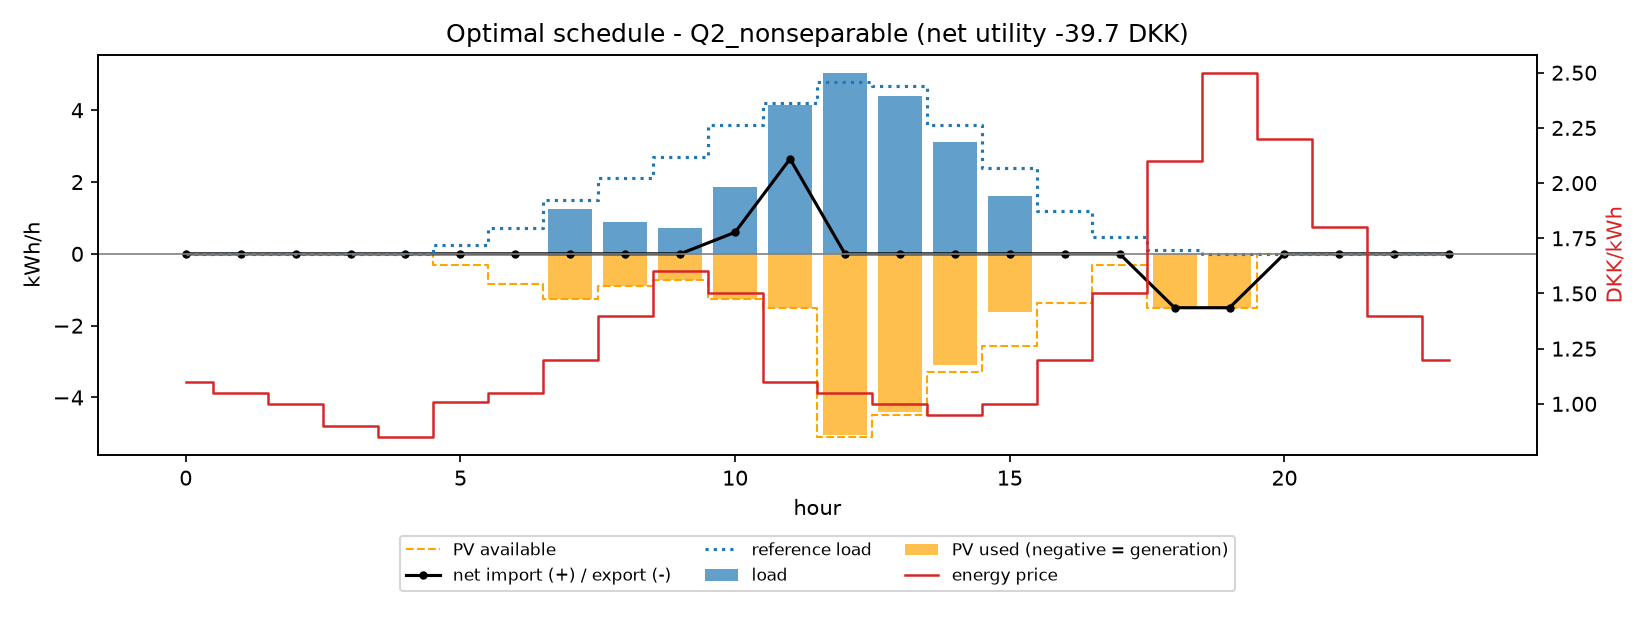
\includegraphics[width=\textwidth]{figures/Q2/q2e_schedule.png}
    \caption{Base case of the accumulated-deviation model ($\rho = 0.8$, $\cQ = 0.05$, $\cS = 0.06$~DKK/kWh$^2$). Same legend as Figure~\ref{fig:q2b_schedule}.}
    \label{fig:q2e_schedule}
\end{figure}

\begin{itemize}
    \item \textbf{Where the deviations occur:} mainly in hours 8--10 ($-1.20$, $-1.98$ and $-1.74$~kWh), where the accumulated deviation grows to $-4.59$~kWh. Hours 5, 6 and 16--18 are at $\Lmin = 0$.
    \item \textbf{Recovery:} after that the load returns close to the reference (hours 11--13: $-0.05$, $+0.25$ and $-0.27$~kWh), and in hour 12 it is above the reference, which is not  possible in 2.(b) and 2.(c). The consumer uses it to reduce the accumulated deviation.
    \item \textbf{Difference with 2.(c):} there the deviation was about $-0.7$~kWh in every hour from 6 to 16, evenly spread. Here it is concentrated in a few hours and then compensated, because sustained deviations cost more than the same energy spread out.
\end{itemize}

\begin{figure}[H]
    \centering
    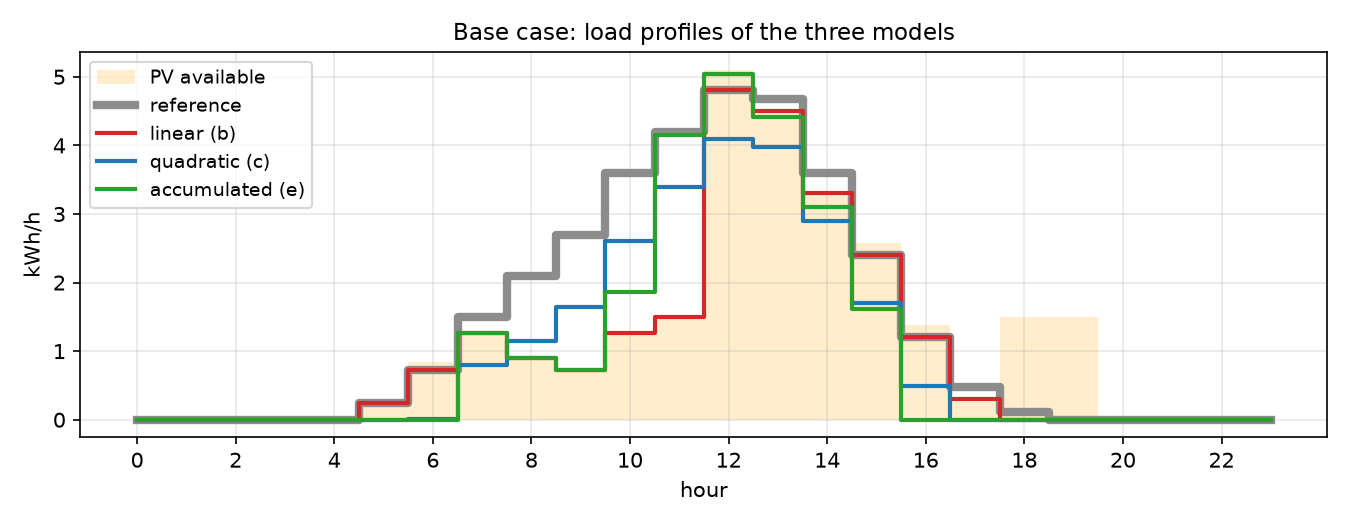
\includegraphics[width=\textwidth]{figures/Q2/q2e_profiles.png}
    \caption{Base case: load profiles of the three models.}
    \label{fig:q2e_profiles}
\end{figure}

\begin{table}[H]
    \centering
    \small
    \begin{tabular}{lrrrrr}
        \toprule
        Model & Cost & Disutility & Energy & $\sum_t |\Delta_t|$ & Hours above \\
              & (DKK) & (DKK) & (kWh) & (kWh) & ref. \\
        \midrule
        Linear (b)       & 31.10 & 13.21 & 23.10 & 9.24 & 0 \\
        Quadratic (c)    & 32.54 &  7.43 & 22.77 & 9.57 & 0 \\
        Accumulated (e)  & 31.90 &  7.85 & 23.06 & 9.77 & 1 \\
        \bottomrule
    \end{tabular}
    \caption{Base case of the three models. The disutilities have different forms, so they are not directly comparable.}
    \label{tab:q2e_base}
\end{table}

\subsubsection{(iv) Effect of the temporal structure of the prices}

\paragraph{Experiment.} We solve the models of 2.(b), 2.(c) and 2.(e) with three price profiles that have the same mean price (1.32~DKK/kWh) and the same values, $\pm 0.8$ around the
mean (12 hours at each), and differ only in the order: \emph{flat} (no variation), \emph{alternating} (high and low every hour) and \emph{blocks} (4 hours high, 4 hours low). The
reference, PV and tariffs are those of the base case.

\paragraph{Why it is a fair comparison.}
\begin{itemize}
    \item \textbf{Across price profiles:} the mean, the amplitude and the set of prices are the same, so only the order changes. The amplitude keeps $\pexp > 0$ ($p_t \geq 0.52 > \tauexp$).
    \item \textbf{Across models:} the coefficients are the base ones, which give a similar deviation on the flat profile (9.12, 9.41 and 9.59~kWh). The surplus is compared as the
    gain with respect to the same model on the flat profile, because the disutilities have different forms and their levels are not comparable.
    \item \textbf{Limitation:} changing the order also changes which hours coincide with the PV and the reference. The separable model of 2.(c) is the benchmark for this effect: whatever it shows is not due to temporal coupling.
\end{itemize}

\begin{table}[H]
    \centering
    \small
    \begin{tabular}{llrrrr}
        \toprule
        Prices & Model & Surplus & Gain vs flat & $\sum_t |\Delta_t|$ & Hours above \\
               &       & (DKK) & (DKK) & (kWh) & ref. \\
        \midrule
        Flat          & Linear      & $-45.78$ &  0.00 &  9.12 & 0 \\
                      & Quadratic   & $-41.29$ &  0.00 &  9.41 & 0 \\
                      & Accumulated & $-41.35$ &  0.00 &  9.59 & 1 \\
        \midrule
        Alternating   & Linear      & $-35.18$ & 10.61 & 16.14 & 0 \\
                      & Quadratic   & $-34.74$ &  6.55 &  9.20 & 0 \\
                      & Accumulated & $-30.39$ & 10.95 & 19.83 & 5 \\
        \midrule
        Blocks of 4 h & Linear      & $-36.07$ &  9.71 & 14.40 & 0 \\
                      & Quadratic   & $-37.52$ &  3.77 &  9.89 & 0 \\
                      & Accumulated & $-33.29$ &  8.06 & 14.31 & 3 \\
        \bottomrule
    \end{tabular}
    \caption{Daily surplus and total deviation for the three price profiles. The surplus is minus the procurement cost minus the disutility.}
    \label{tab:q2e_experiment}
\end{table}

\begin{figure}[H]
    \centering
    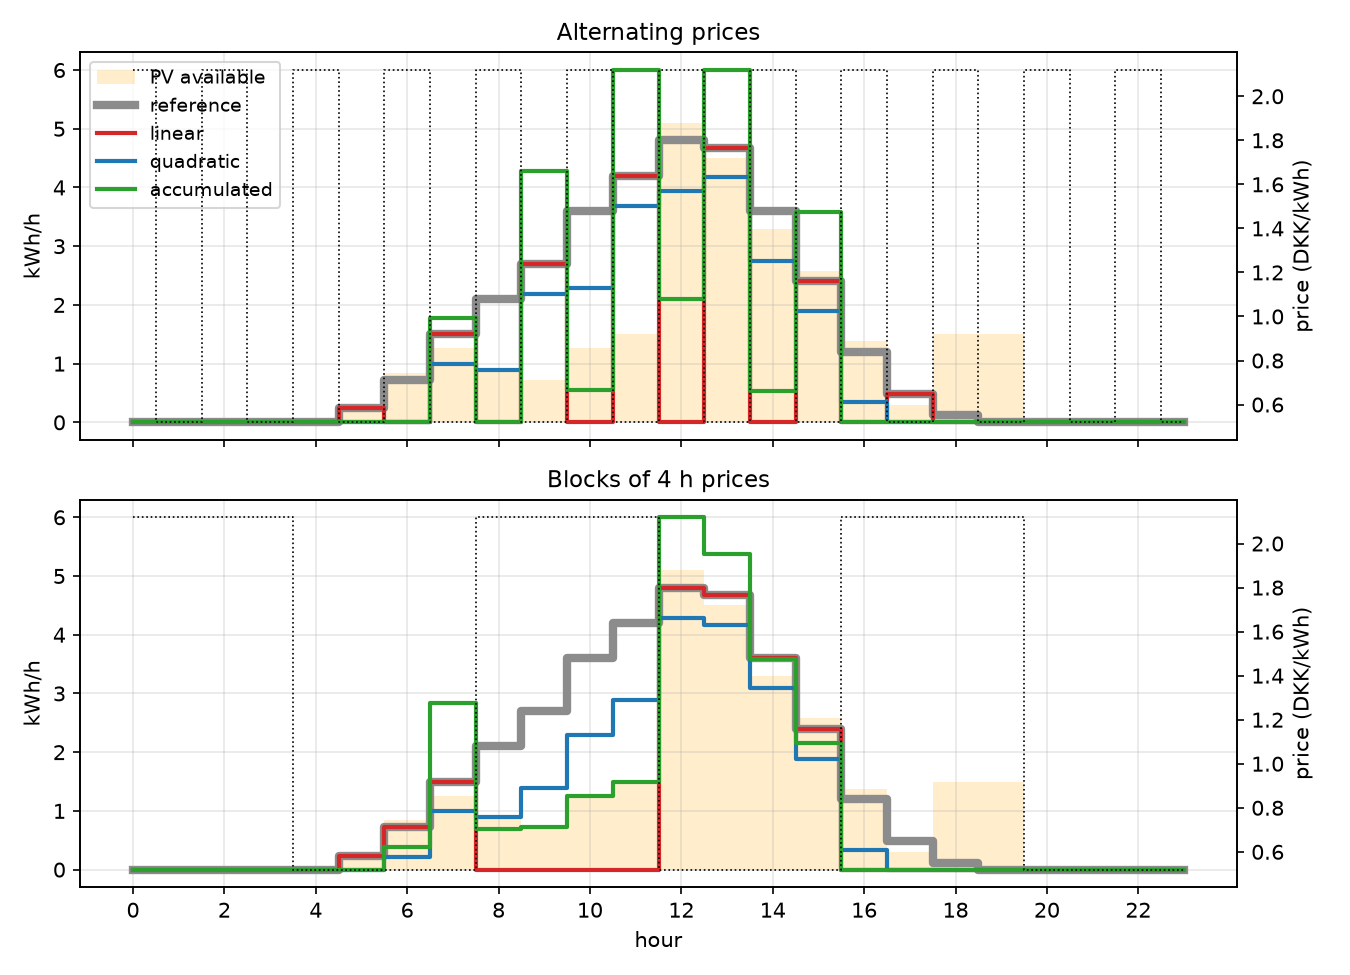
\includegraphics[width=\textwidth]{figures/Q2/q2e_experiment.png}
    \caption{Load of the three models under alternating prices (top) and blocks of 4 hours (bottom). The dotted line is the price.}
    \label{fig:q2e_experiment}
\end{figure}

\paragraph{Results.}
\begin{itemize}
    \item \textbf{Quadratic (c):} it hardly reacts to the order of the prices: the deviation is 9.20~kWh with alternating prices and 9.89~kWh with blocks. Its different gain (6.55 vs 3.77~DKK) comes from the pairing of cheap hours with the PV and the reference.
    \item \textbf{Accumulated (e):} with alternating prices it deviates twice as much (19.83~kWh) and goes above the reference in 5 hours: it consumes less in the expensive hours and compensates in the cheap ones (Figure~\ref{fig:q2e_experiment}), so the accumulated deviation stays small. With blocks it cannot compensate inside a 4-hour block, and the deviation is smaller (14.31~kWh), with fewer hours above the reference (3) and a lower gain (8.06 vs 10.95~DKK).
    \item \textbf{Linear (b):} it also deviates more with alternating prices, but because of its thresholds (the high prices are above $\cL$), not because of the temporal coupling.
    \item \textbf{Surplus:} the advantage of alternating over blocks is similar for (c) and (e) (2.8 and 2.9~DKK), so in the surplus the pairing effect dominates. The temporal coupling shows in how the consumer gets there: shifting load between hours.
\end{itemize}

\newpage
\section{Question 3}
% Question 3 -- draft so far. 3.(a): definitions and daily problem are written (they only restate
% the brief); the properties (problem class, convexity, feasibility) are left as TODO with hints.
%
% NOTE ON 2.(c): Question 3 starts from the quadratic disutility of 2.(c), which is not written
% yet. Below the disutility is kept generic, D_t(l_t), as in 2.(a) (convex, differentiable). This
% is enough to write 3.(b): the KKT conditions only need D_t'(l_t). Once 2.(c) is written, D_t is
% replaced by the quadratic disutility and the properties below are specialised.
%
% 3.(c) (qualitative hypotheses), Ignacio's note: the reasoning -- does the consumer ever
% consume above its hourly reference, and above E^min -- follows from a cost-benefit argument
% (disutility of deviating vs. cost/benefit of importing/exporting), not from duality, so it
% does not need 2.(c) to be implemented. Not written yet.

\subsection{(a) Formulation with a minimum daily energy}

\subsubsection{New input data and constraint}
Starting from the model of Question~2.(c), the consumer must now consume at least a minimum
total energy $\Emin$ (kWh) over the whole day. This is the only new input datum, and it adds a
single new constraint:
\begin{equation}
    \sum_{t \in \T} \load \geq \Emin.
    \label{eq:c_min_energy}
\end{equation}
No new decision variables are needed.
\subsubsection{Daily problem}
The daily problem keeps the objective of Question~2 and all the constraints of Question~1, and
adds \eqref{eq:c_min_energy}. With $D_t$ the disutility of the deviation of the load from the
reference $\lref$ (in Question~3, the quadratic disutility of 2.(c)):
\begin{align}
    \max_{\{\load, \qimp, \qexp, \pvprod\}_{t \in \T}} \quad
    & \sum_{t \in \T} \Big( - D_t(\load) - \pimp \, \qimp + \pexp \, \qexp - \cpv \, \pvprod \Big)
    \label{eq:q3_objective} \\
    \text{s.t.} \quad
    & \load = \pvprod + \qimp - \qexp, & \forall t \in \T, \nonumber \\
    & \Lmin \leq \load \leq \Lmax, & \forall t \in \T, \nonumber \\
    & 0 \leq \pvprod \leq \PVmax, & \forall t \in \T, \nonumber \\
    & \qimp \geq 0, \quad \qexp \geq 0, & \forall t \in \T, \nonumber \\
    & \sum_{t \in \T} \load \geq \Emin. & \nonumber
\end{align}

\subsubsection{Change in the properties}
\begin{itemize}
    \item \textbf{Decomposability:} constraint \eqref{eq:c_min_energy} is the first constraint
    of the assignment that links different hours, since it involves the loads of all 24 hours. The daily problem can therefore no longer be split into 24 independent hourly
    problems: it has to be solved as a single 24-hour problem.
    \item \textbf{Problem class and convexity:}
    The objective is the same as in Question~2.(c), where the quadratic disutility gives a concave quadratic objective. The hourly constraints are affine, including  the new constraint \eqref{eq:c_min_energy}. The problem therefore remains a convex Quadratic Program (QP). So the new constraint impacts decomposability but not the convexity. 

    \item \textbf{Feasibility:}
The largest total energy the consumer can consume during the day is $24\Lmax$. The problem is therefore feasible as long as $\Emin \leq 24\Lmax$, assuming $\Lmin \leq \Lmax$ and that the original hourly constraints are feasible. The reference profile $\lref$ does not restrict feasibility, since it only appears in the objective through the disutility. The load may therefore deviate from $\lref$ if this is needed to satisfy \eqref{eq:c_min_energy}.

\end{itemize}

\subsection{(b) Lagrangian, dual problem and KKT conditions of the daily problem}
% HINTS (not final text) for whoever writes 3.(b):
% - Set up as in 1.(b): minimisation, h(x) = 0 and g(x) <= 0, one multiplier per constraint. The
%   hourly multipliers of 1.(b) are reused (macros \lbal, \muLlo, ..., all with the hour index t);
%   the new one is \muE (already in main.tex), a single scalar for the whole day.
% - The Lagrangian is the sum over t of the hourly terms of 1.(b), with D_t in place of the
%   linear utility, plus the term of the minimum-energy constraint.
% - In the stationarity condition of the load, D_t'(l_t) appears and \muE appears in every
%   hour: this is how the multiplier couples the hours in the KKT conditions.
% - Strong duality and necessity/sufficiency of KKT: same route as in 1.(b) (problem class from
%   (a), Slater's condition reduces to feasibility when the constraints are affine), and the
%   feasibility condition of 3.(a) is what is needed here.
Following the brief, the multiplier of the minimum-energy constraint \eqref{eq:c_min_energy}
is denoted by $\muE \geq 0$. It is a multiplier of the same kind as those of Question~1.(b):
it belongs to an inequality, which in the form $g(x) \leq 0$ reads
$\Emin - \sum_{t \in \T} \load \leq 0$, and it is in DKK/kWh. Unlike the hourly multipliers, it
has no hour index, since the constraint applies to the whole day.

\subsubsection{Lagrangian}

As in Question~1.(b), we write the problem in minimization form. The objective
then becomes the negative of \eqref{eq:q3_objective}. The Lagrangian is

\begin{equation}
\begin{aligned}
\mathcal{L}
= \sum_{t\in\T} \Big[
& D_t(\load)
+ \pimp\,\qimp
- \pexp\,\qexp
+ \cpv\,\pvprod \\
&+ \lbal(\load-\pvprod-\qimp+\qexp) \\
&+ \muLlo(\Lmin-\load)
+ \muLup(\load-\Lmax) \\
&- \muPVlo\pvprod
+ \muPVup(\pvprod-\PVmax) \\
&- \muimp\qimp
- \muexp\qexp
\Big] \\
&+ \muE
\left(
\Emin-\sum_{t\in\T}\load
\right).
\end{aligned}
\label{eq:q3_lagrangian}
\end{equation}
\subsubsection{Dual problem}
The dual function is given when the dual variables are fixed and the Lagrangian is minimized. For the load, the quadratic disutility from 2 c) is $D_t(\load)=c^Q(\load-\lref)^2$. Study the Lagrangian at \eqref{eq:q3_lagrangian} and it can be seen that the terms that depend on the $\load$ are
$D_t(\load)+\lbal\load-\muLlo\load+\muLup\load-\muE\load$. To keep this notation shorter: $\beta_t=\lbal-\muLlo+\muLup-\muE$. Add both of this together and it can be seen that the load dependent part of the Lagrangian becomes $c^Q(\load-\lref)^2+\beta_t\load$.

If we minimize this with respect to $\load$ gives $2c^Q(\load-\lref)+\beta_t=0$ which imples: $\load=\lref-\beta_t/(2c^Q)$. If this value is then substituted back into the Lagrangian the load contribution becomes $\beta_t\lref-\beta_t^2/(4c^Q)$.

The remaining primal variables are linear in the Lagrangian. Their bounds have
already been included through their multipliers, so they are treated as free when forming the dual function. If one of their coefficients was non-zero, the Lagrangian could be made infinitely small. The dual function would then be $-\infty$.The required conditions are therefore
$\cpv-\lbal-\muPVlo+\muPVup=0$ for PV,
$\pimp-\lbal-\muimp=0$ for imports, and
$-\pexp+\lbal-\muexp=0$ for exports, for every $t\in\T$.

After minimizing over all primal variables, the dual function is

\begin{equation}
\begin{aligned}
q(\boldsymbol{\lambda},\boldsymbol{\mu},\muE)
=
\muE\Emin
+
\sum_{t\in\T}
\left[
    \muLlo\Lmin
    -\muLup\Lmax
    -\muPVup\PVmax
    +\beta_t\lref
    -\frac{\beta_t^2}{4c^Q}
\right].
\end{aligned}
\label{eq:q3_dual_function}
\end{equation}

This expression is finite only when the three coefficient conditions above hold. Otherwise
$q(\boldsymbol{\lambda},\boldsymbol{\mu},\muE)=-\infty$.

The dual problem is therefore

\begin{align}
\max_{\boldsymbol{\lambda},\boldsymbol{\mu},\muE}
\quad
& q(\boldsymbol{\lambda},\boldsymbol{\mu},\muE)
\label{eq:q3_dual_problem} \\
\text{s.t.}\quad
& \cpv-\lbal-\muPVlo+\muPVup=0,
&& \forall t\in\T, \nonumber\\
& \pimp-\lbal-\muimp=0,
&& \forall t\in\T, \nonumber\\
& -\pexp+\lbal-\muexp=0,
&& \forall t\in\T, \nonumber\\
& \muLlo,\muLup,\muPVlo,\muPVup,\muimp,\muexp\geq0,
&& \forall t\in\T. \nonumber
\end{align}

Also $\muE\geq0$, while $\lbal$ is free for every $t\in\T$.

\subsubsection{KKT conditions}
Primal feasibility, dual feasibility, stationarity and complementary slackness will be shown below:

\paragraph{Primal feasibility}
The primal variables must satisfy the constraints of Q3 a. So: 

$\load=\pvprod+\qimp-\qexp$, $\Lmin\leq\load\leq\Lmax$,
$0\leq\pvprod\leq\PVmax$, and $\qimp,\qexp\geq0$ for every $t\in\T$.
The daily minimum-energy requirement must also hold, so
$\sum_{t\in\T}\load\geq\Emin$.

\paragraph{Dual feasibility.}
All multipliers of inequality constraints must be non-negative. For every $t\in\T$,
the load and PV multipliers satisfy
$\muLlo,\muLup,\muPVlo,\muPVup\geq0$.
The import and export multipliers satisfy $\muimp,\muexp\geq0$, and the daily
multiplier satisfies $\muE\geq0$. The power-balance multiplier $\lbal$ is free.


\paragraph{Stationarity.}
The derivative of the Lagrangian with respect to each primal variable must be zero. This gives

\begin{align}
    \frac{\partial \mathcal{L}}{\partial \load}
    &= 2c^Q(\load-\lref)+\lbal-\muLlo+\muLup-\muE = 0,
    && \forall t\in\T,
    \label{eq:q3_stationarity_load}\\
    \frac{\partial \mathcal{L}}{\partial \pvprod}
    &= \cpv-\lbal-\muPVlo+\muPVup = 0,
    && \forall t\in\T, \nonumber\\
    \frac{\partial \mathcal{L}}{\partial \qimp}
    &= \pimp-\lbal-\muimp = 0,
    && \forall t\in\T, \nonumber\\
    \frac{\partial \mathcal{L}}{\partial \qexp}
    &= -\pexp+\lbal-\muexp = 0,
    && \forall t\in\T. \nonumber
\end{align}

\paragraph{Complementary slackness} Multiplier times constraint must be zero:
\begin{align}
    \muLlo(\Lmin-\load) &= 0,
    && \forall t\in\T, \nonumber\\
    \muLup(\load-\Lmax) &= 0,
    && \forall t\in\T, \nonumber\\
    \muPVlo\pvprod &= 0,
    && \forall t\in\T, \nonumber\\
    \muPVup(\pvprod-\PVmax) &= 0,
    && \forall t\in\T, \nonumber\\
    \muimp\qimp &= 0,
    && \forall t\in\T, \nonumber\\
    \muexp\qexp &= 0,
    && \forall t\in\T, \nonumber\\
    \muE\left(\Emin-\sum_{t\in\T}\load\right) &= 0.
    \label{eq:q3_complementary}
\end{align}

\subsubsection{Strong duality}

The formulation in 3 a of the daily problem is a convex quadratic problem and all constraints are affine. Given that all constraints are affine, the slater argument from Q1 (b) can be recycled. So for that reason strong duality holds here also. Optimal objective value is same for both primal and dual and KKT conditions are sufficient and necessary for optimality.

\subsubsection{(c) Expected behavior}
\paragraph{Can the consumer consume above it hourly reference?}
Yes it can. Partly because it can be forced to do so to fit its minimum daily energy demand $\Emin>\sum_{t\in\T}\lref$. This could make it such that in the cheaper hours it deviates more above the reference compared to the more expensive hours, where the reference is kept.

\paragraph{Can the consumer consume above its daily minimum requirement?}
Yes this is also possible. $\Emin$ only sets a lower bound and not an upper one. So if electricity is cheap and it increases utility more than it costs the consumer can consume above it daily requirement $\Emin$.

\subsubsection{(d) model implementation}
The necessary changes for making the model work can be found in the repository.
\subsubsection{(e) Hourly Scheduled compared to 2c}

\begin{figure}[H]
    \centering
    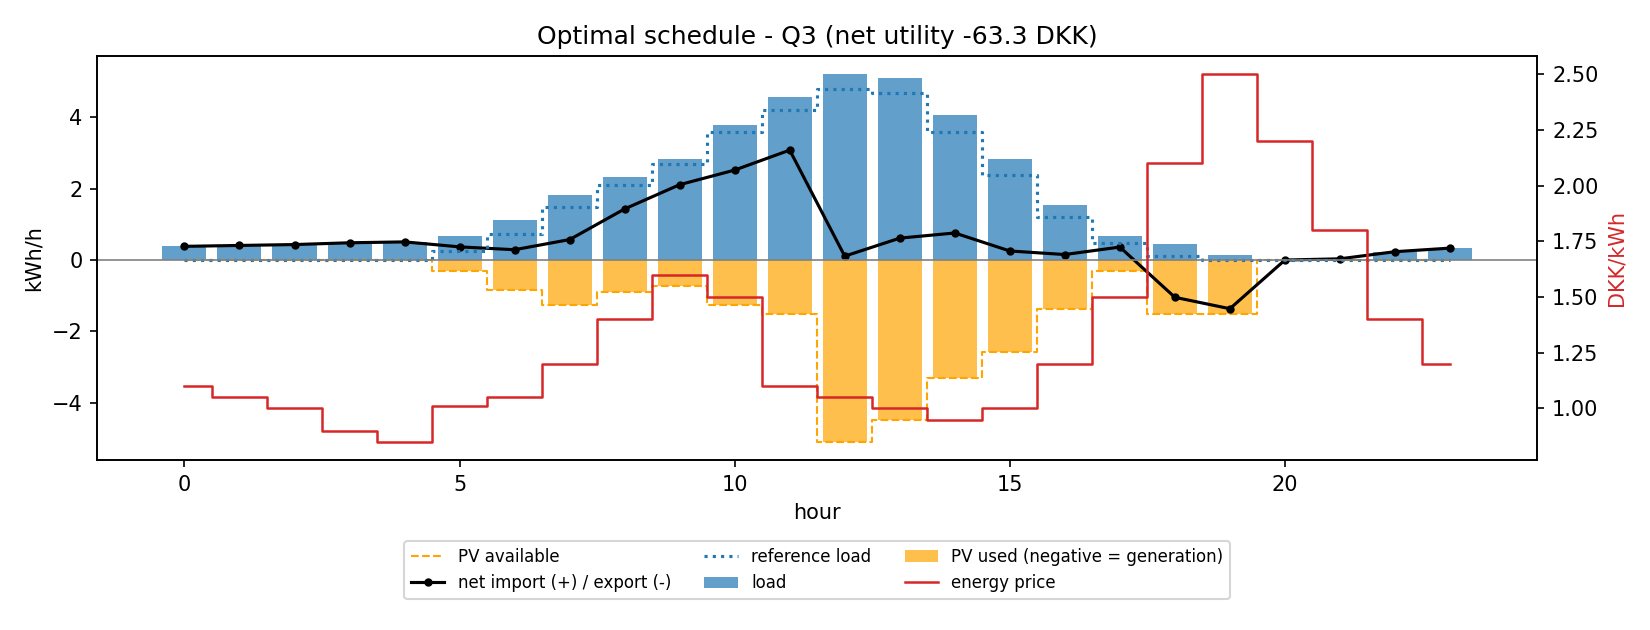
\includegraphics[width=\textwidth]{figures/Q3/schedule.png}
    \caption{Caption for the first plot.}
    \label{fig:q3_plot1}
\end{figure}

\begin{figure}[H]
    \centering
    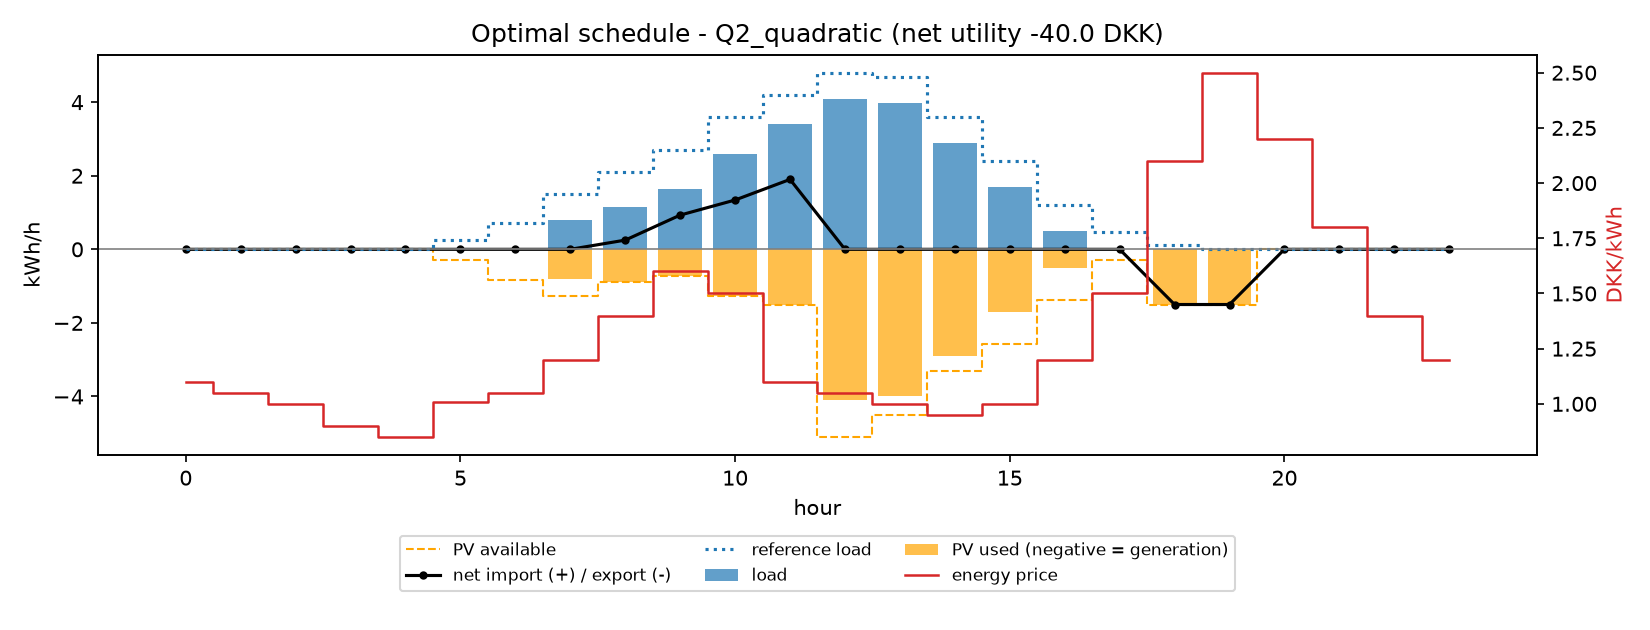
\includegraphics[width=\textwidth]{figures/Q2/q2c_schedule.png}
    \caption{Caption for the second plot.}
    \label{fig:q3_plot2}
\end{figure}
\subsection{(g) A small battery}

\subsubsection{(i) Formulation with a battery}
The model of (a) is kept, with the same objective and constraints, and a battery is added. Its
data are given in the repository; since the time step is one hour, a power in kW is
equivalent to an energy of kWh per hour.

\paragraph{New input data.}
\begin{itemize}
    \item $\Ebat$: energy capacity of the battery, 4~kWh.
    \item $\Pch$, $\Pdis$: maximum charging and discharging power, 1.5~kW each.
    \item $\etach$, $\etadis$: charging and discharging efficiencies, 0.95 each. $\etach$ is the
    fraction of the charged energy that reaches the battery, and $\etadis$ the fraction of the
    discharged energy that reaches the consumer.
    \item $\einit$: state of charge at the start of the day, 2~kWh (50\,\% of $\Ebat$).
\end{itemize}

\paragraph{New decision variables.}
\begin{itemize}
    \item $\pch \geq 0$, $\pdis \geq 0$: energy charged into and discharged from the battery in
    hour $t$ (kWh/h), measured on the consumer's side.
    \item $\soc$: state of charge at the end of hour $t$ (kWh).
\end{itemize}

\paragraph{New and modified constraints.}
The power balance of (a) now includes the battery, which acts as an extra load when charging
and as an extra source when discharging:
\begin{equation}
    \load + \pch = \pvprod + \qimp - \qexp + \pdis, \qquad \forall t \in \T.
    \label{eq:g_balance}
\end{equation}
The state of charge links each hour with the previous one, with the losses of both
conversions:
\begin{equation}
    \soc = \soc[t-1] + \etach \, \pch - \frac{\pdis}{\etadis}, \qquad \forall t \in \T,
    \qquad \text{with } \soc[-1] = \einit.
    \label{eq:g_soc}
\end{equation}
The state of charge and the power are limited by the battery data:
\begin{align}
    & 0 \leq \soc \leq \Ebat, & \forall t \in \T, \label{eq:g_cap} \
    & 0 \leq \pch \leq \Pch, \quad 0 \leq \pdis \leq \Pdis, & \forall t \in \T. \label{eq:g_power}
\end{align}
The minimum-energy requirement \eqref{eq:c_min_energy} is unchanged: it applies to the load
$\load$, so the energy that the battery delivers to the load counts towards $\Emin$, while
the energy stored in the battery or lost in it does not.

\paragraph{State of charge at the end of the day.}
We require the battery to end the day with at least its initial energy:
\begin{equation}
    \soc[23] \geq \einit.
    \label{eq:g_end}
\end{equation}
With this condition the battery cannot sell or consume the energy it started with, so the
value of the battery measured in (iv) and (v) only comes from moving energy between hours,
and the comparison with the case without battery is fair. It also avoids choosing a price for
the energy left at the end of the day. We expect the battery to discharge during the evening
peak and to recharge in the cheapest hours after it, so that it reaches $\einit$ at hour 23.

Two alternatives were considered. Without any condition on $\soc[23]$, the energy left after
hour 23 has no value for the model, so the battery empties itself during the evening peak and
does not recharge; this overestimates its value with energy it did not earn. Valuing the final
energy in the objective, $+\pi^{\mathrm{end}} \soc[23]$, is more realistic, but the right
value of $\pi^{\mathrm{end}}$ is what that energy saves at the next price peak of the
following day, not the price at midnight, so it would have to be estimated. (Taking the last
price $p_{23}$ or the falling trend of the night would make recharging unprofitable, given
the losses $\etach \etadis < 1$.) Depending on $\pi^{\mathrm{end}}$, the battery would then end
the day full or empty.

\paragraph{Properties.}
The objective is unchanged and all the new constraints are affine, so the problem is still a
convex QP. It is feasible under the same condition as in (a), since leaving the battery idle
($\pch = \pdis = 0$, $\soc = \einit$) satisfies all the battery constraints. The state of
charge \eqref{eq:g_soc} adds a second link between consecutive hours, besides $\Emin$, so the
problem still does not decompose by hour.

% IDEA for (iv) or (v), extra analysis: compare numerically the end condition (eq:g_end) with
% (1) a 48-hour horizon using the next-day data of the repository (energy_price_next_day,
% pv_available_next_day, reference_load_next_day), keeping only the first 24 hours, and
% (2) a value pi^end on the final energy taken from the next-day peak. Shows how much the
% end-of-horizon choice changes the schedule of the last hours and the value of the battery.

\subsubsection{(ii) Simultaneous charging and discharging}
\paragraph{With the data of this assignment.}
Charging and discharging in the same hour is never optimal. Suppose that in some hour both
$\pch > 0$ and $\pdis > 0$, and reduce them together, $\pch$ by a small $\delta > 0$ and $\pdis$ by
$\etach \etadis \, \delta$. By \eqref{eq:g_soc} the state of charge $\soc$ does not change, so
no other hour is affected. In the balance \eqref{eq:g_balance}, however, the battery now
draws $(1 - \etach \etadis)\,\delta > 0$ less energy: this is the energy that was being lost
in the round trip. That energy can be used to import less, saving $\pimp > 0$, to export
more, earning $\pexp > 0$, or to produce less PV, saving $\cpv > 0$. Exporting more is always
possible, since exports are unbounded, so the objective strictly improves in every hour,
whatever the regime. With our data $\etach \etadis = 0.9025 < 1$, all effective prices are
positive ($\pexp \geq 0.85 - 0.40 = 0.45$~DKK/kWh) and the PV can be curtailed, so wasting
energy in the battery always costs money.

\paragraph{When it becomes a real risk.}
The argument fails when losing energy is no longer a cost: when importing is paid
($\pimp < 0$), or when exporting costs money ($\pexp < 0$) and a surplus cannot be curtailed
or used by the load. Burning energy through simultaneous charging and discharging then
becomes profitable. With a lossless battery
($\etach = \etadis = 1$) the overlap costs nothing: the optimum is not unique, and the solver
may return a solution with overlap.

\paragraph{How it could be fixed.}
The exact fix is a binary variable $z_t \in \{0, 1\}$ that allows only one direction per hour,
\begin{equation}
    \pch \leq \Pch \, z_t, \qquad \pdis \leq \Pdis \, (1 - z_t), \qquad \forall t \in \T,
\end{equation}
which turns the QP into a mixed-integer QP (MIQP), harder to solve and without duals. A
cheaper mitigation is a linear degradation cost $c^{\mathrm{deg}} (\pch + \pdis)$ in the
cost, which makes every kWh through the battery more expensive. It acts like extra losses: it
removes the overlap only as long as the gain from burning energy is smaller than the cost, so
with very negative prices the overlap can still appear.


\newpage
\section{Appendix A} \label{ch6}

All input data of the base cases are those of the repository. The table below lists the values
that were chosen by the group. They are also set in the source code
(\texttt{main.py} and \texttt{src/}), so every result can be reproduced with the commands given in
each section.

\begin{table}[H]
\centering
\small
\begin{tabularx}{\textwidth}{llX}
\toprule
\textbf{Question} & \textbf{Parameter} & \textbf{Chosen values} \\
\midrule
2.(b).iv & Sweep of $c^{L}$ & 0.005 to 3.195~DKK/kWh in steps of 0.01 (offset by 0.005 so that no run lies on a price threshold) \\
2.(c).iv & Sweep of $c^{Q}$ & 0.01 to 3.20~DKK/kWh$^2$ in steps of 0.01 \\
2.(d) & Scenarios & Base: $c^{L} = 1.43$~DKK/kWh, $c^{Q} = 1.00$~DKK/kWh$^2$; low: $c^{L} = c^{Q} = 0.50$; high: $c^{L} = c^{Q} = 3.20$; Question~1 model with $\uL = c^{L}$ \\
2.(e) & Disutility parameters & $\rho = 0.8$, $c^{Q} = 0.05$~DKK/kWh$^2$, $c^{S} = 0.06$~DKK/kWh$^2$ \\
2.(e).iv & Price profiles & Mean of the base prices (1.32~DKK/kWh); flat; alternating $\pm 0.8$~DKK/kWh every hour; blocks of 4~h at $\pm 0.8$~DKK/kWh \\
\midrule
3.(f) & $\Emin$ & 20, 30, 40, 80~kWh \\
3.(f) & $c^{Q}$ & 0.1, 1, 5~DKK/kWh$^2$ (with $\Emin = 40$~kWh) \\
3.(f) & $\Lmax$ & 7, 3.5, 1.7~kWh/h (with $\Emin = 40$~kWh) \\
\midrule
3.(g).i & Morning peak of $D+1$ & Searched in hours 0--11 of the following day, \eqref{eq:g_piend} \\
3.(g).v & Price spread & 0, 0.5, 1, 1.5, 2 times the base spread, same mean, on both days \\
3.(g).v & Price level & $-0.5$, 0, 0.5, 1.0~DKK/kWh added to all prices, on both days \\
3.(g).v & $c^{Q}$ & 0.02, 0.1, 0.3, 1, 3, 10~DKK/kWh$^2$ \\
3.(g).v & Capacity $\Ebat$ & 1, 2, 4, 8, 16~kWh, with $\einit$ at 50\,\% of it \\
3.(g).v & Power $\Pch = \Pdis$ & 0.5, 1, 1.5, 3, 6~kW \\
3.(g).v & Efficiency $\etach = \etadis$ & 0.80, 0.85, 0.90, 0.95, 1.00 \\
3.(g).v & End of the day & Trend $\pimp[23] + (\pimp[23] - \pimp[22])$; last price $\pimp[23]$; $\pimp[23]/\etach$; free end; cyclic; $\piend$ from 1.40 to 2.00~DKK/kWh in steps of 0.01 \\
3.(g).v & Benchmark & Day $D$ and hours 0--10 of $D+1$; $\Emin$ on day $D$ only; no value for the energy left at the end \\
\bottomrule
\end{tabularx}
\caption{Values chosen by the group.}
\label{tab:appendix}
\end{table}


\label{endOfDoc}
\label{EndOfText}
\end{document}
